\documentclass{beamer}

\usetheme{Warsaw}
%\usetheme{CambridgeUS}

% modification history
% created on 18 sep 2011
% modified on 25 mar

%\usepackage{amsfonts, amsmath, amssymb}

%\setbeamertemplate{theorems}[numbered]
%\setbeamertemplate{theorems}[ams style] 
\usepackage[skins,breakable]{tcolorbox}
%\usepackage[normalem]{ulem}

%\usefonttheme[onlymath]{serif}                     // change the style of math font 

%=============set slide number=================
\addtobeamertemplate{navigation symbols}{}{
    \usebeamerfont{footline}
    \usebeamercolor[fg]{footline}
    \hspace{1em}
    \insertframenumber/\inserttotalframenumber
}
\setbeamercolor{footline}{fg=black}
\setbeamerfont{footline}{series=\bfseries}


%=============set footline=====================
\setbeamertemplate{footline}
{
  \leavevmode%
  \hbox{%
  \begin{beamercolorbox}[wd=.55\paperwidth,ht=2.25ex,dp=1ex,center]{author in head/foot}%
    \usebeamerfont{author in head/foot}\insertshortauthor
  \end{beamercolorbox}%
  \begin{beamercolorbox}[wd=.45\paperwidth,ht=2.25ex,dp=1ex,center]{title in head/foot}%
    \usebeamerfont{title in head/foot}\insertshorttitle
  \end{beamercolorbox}}%
  \vskip0pt%
}

%creating a rectangle box def
\newtcbox{\mybox}[1][red]{arc=0pt,outer arc=0pt,colback=#1!10!white,colframe=#1!50!black, boxsep=0pt,left=1pt,right=1pt,top=2pt,bottom=2pt,boxrule=0pt,bottomrule=1pt,toprule=1pt}

\newtcbox{\xmybox}[1][red]{arc=7pt,colback=#1!10!white,colframe=#1!50!black,before upper={\rule[-3pt]{0pt}{10pt}},boxrule=1pt,boxsep=0pt,left=6pt,right=6pt,top=2pt,bottom=2pt}
%the ``on line'' option doesn't work. so omitting it

%===== spacing =====

\def\extraspacing{\vspace{2mm} \noindent}
\def\vgap{\vspace{2mm}}
\def\hgap{\textrm{\hspace{1mm}}}

%===== tabbing =====

\def\tab{\hspace{2mm}}
\def\tabpos{\hspace{4mm} \= \hspace{4mm} \= \hspace{4mm} \= \hspace{4mm} \=
\hspace{4mm} \= \hspace{4mm} \= \hspace{4mm} \= \hspace{4mm} \= \hspace{4mm}
\kill}
\newcommand{\mytab}[1]{\begin{tabbing}\tabpos #1\end{tabbing}}

%===== blocks =====

% \newtheorem{theorem}{Theorem}
% \newtheorem{lemma}{Lemma}
% \newtheorem{corollary}{Corollary}
% \newtheorem{proposition}{Proposition}
% \newtheorem{definition}{Definition}
% \newtheorem{problem}{Problem}

\newcommand{\cbox}[2]{\begin{tcolorbox}[arc=0mm, colframe=#1!50!black, colback=#1!10!white]#2\end{tcolorbox}}
\newcommand{\minipg}[2]{\begin{center}\begin{minipage}{#1}#2\end{minipage}\end{center}}
\newcommand{\myfrm}[1]{\begin{frame}\begin{small}#1\end{small}\end{frame}} 
\newcommand{\myitems}[1]{\begin{itemize}#1\end{itemize}}
\newcommand{\myenums}[1]{\begin{enumerate}#1\end{enumerate}}
\newcommand{\myfig}[1]{\begin{figure}\centering #1\end{figure}}
    
%===== math macros =====
\newcommand{\bm}[1]{\textrm{\boldmath${#1}$}}
%\newcommand{\smat}[2]{\left[\begin{tabular}{#1}#2\end{tabular}\right]}
%\newcommand{\bmat}[2]{\left|\begin{tabular}{#1}#2\end{tabular}\right|}
\newcommand{\bmat}[1]{\begin{bmatrix}#1\end{bmatrix}}
\newcommand{\vmat}[1]{\begin{vmatrix}#1\end{vmatrix}}
\newcommand{\myeqn}[1]{\begin{eqnarray}#1\end{eqnarray}}
\newcommand{\set}[1]{\{#1\}}

\def\eps{\epsilon}
\def\fr{\frac}
\def\lc{\lceil}
\def\lf{\lfloor}
\def\rc{\rceil}
\def\rf{\rfloor}
\def\Pr{\textrm{\boldmath$Pr$}}
\def\expt{\textrm{\boldmath$E$}}
\def\real{\mathbb{R}}
\def\int{\mathbb{Z}}
\def\*{\star}
\def\tO{\tilde{O}}

\DeclareMathOperator*{\argmin}{arg\,min}
\DeclareMathOperator*{\polylg}{polylg}
\DeclareMathOperator*{\polylog}{polylog}
\DeclareMathOperator*{\intr}{\cap}

\def\nn{\nonumber}
\def\mit{\mathit}


%===== misc =====

\def\done{\hspace*{\fill} $\framebox[2mm]{}$}	% end of proof
\def\ttt{\texttt}

%===== coloring =====
\newcommand{\red}[1]{\textcolor{red}{#1}}
\newcommand{\bred}[1]{\textcolor{red}{\bf #1}}
\newcommand{\blue}[1]{\textcolor{blue}{\bf #1}}

\usepackage{color}
\usepackage{graphicx}
\usepackage{multirow}
\usepackage[skins,breakable]{tcolorbox}

\def\done{\hfill$\square$}
\def\vgap{\vspace{2mm}}


\title{Some Recent Results in Database Theory}
\author[]{Yufei Tao}
\institute[]
{CSE Dept \\ Chinese University of Hong Kong}
\date{}

%\date{}

\begin{document}
%-------------------------------------------------------------
    \begin{frame}
        \titlepage
    \end{frame}
%-------------------------------------------------------------
\myfrm{
    \begin{center}
    This talk aims to give you a flavor of fundamental database research.
    \end{center}
}
%-------------------------------------------------------------
\begin{frame}{} 
\begin{small}
    \begin{center} 
         \mybox[yellow]{I: Machine Learning}
    \end{center}
\end{small}
\end{frame}
%-------------------------------------------------------------
\begin{frame}
\begin{small}
   
%    $\red{P}$: a set of points in multidimensional space. \\
%    Each point has a \blue{label}: either 0 or 1. 

    \xmybox{Classification} 
   
   \begin{center}
       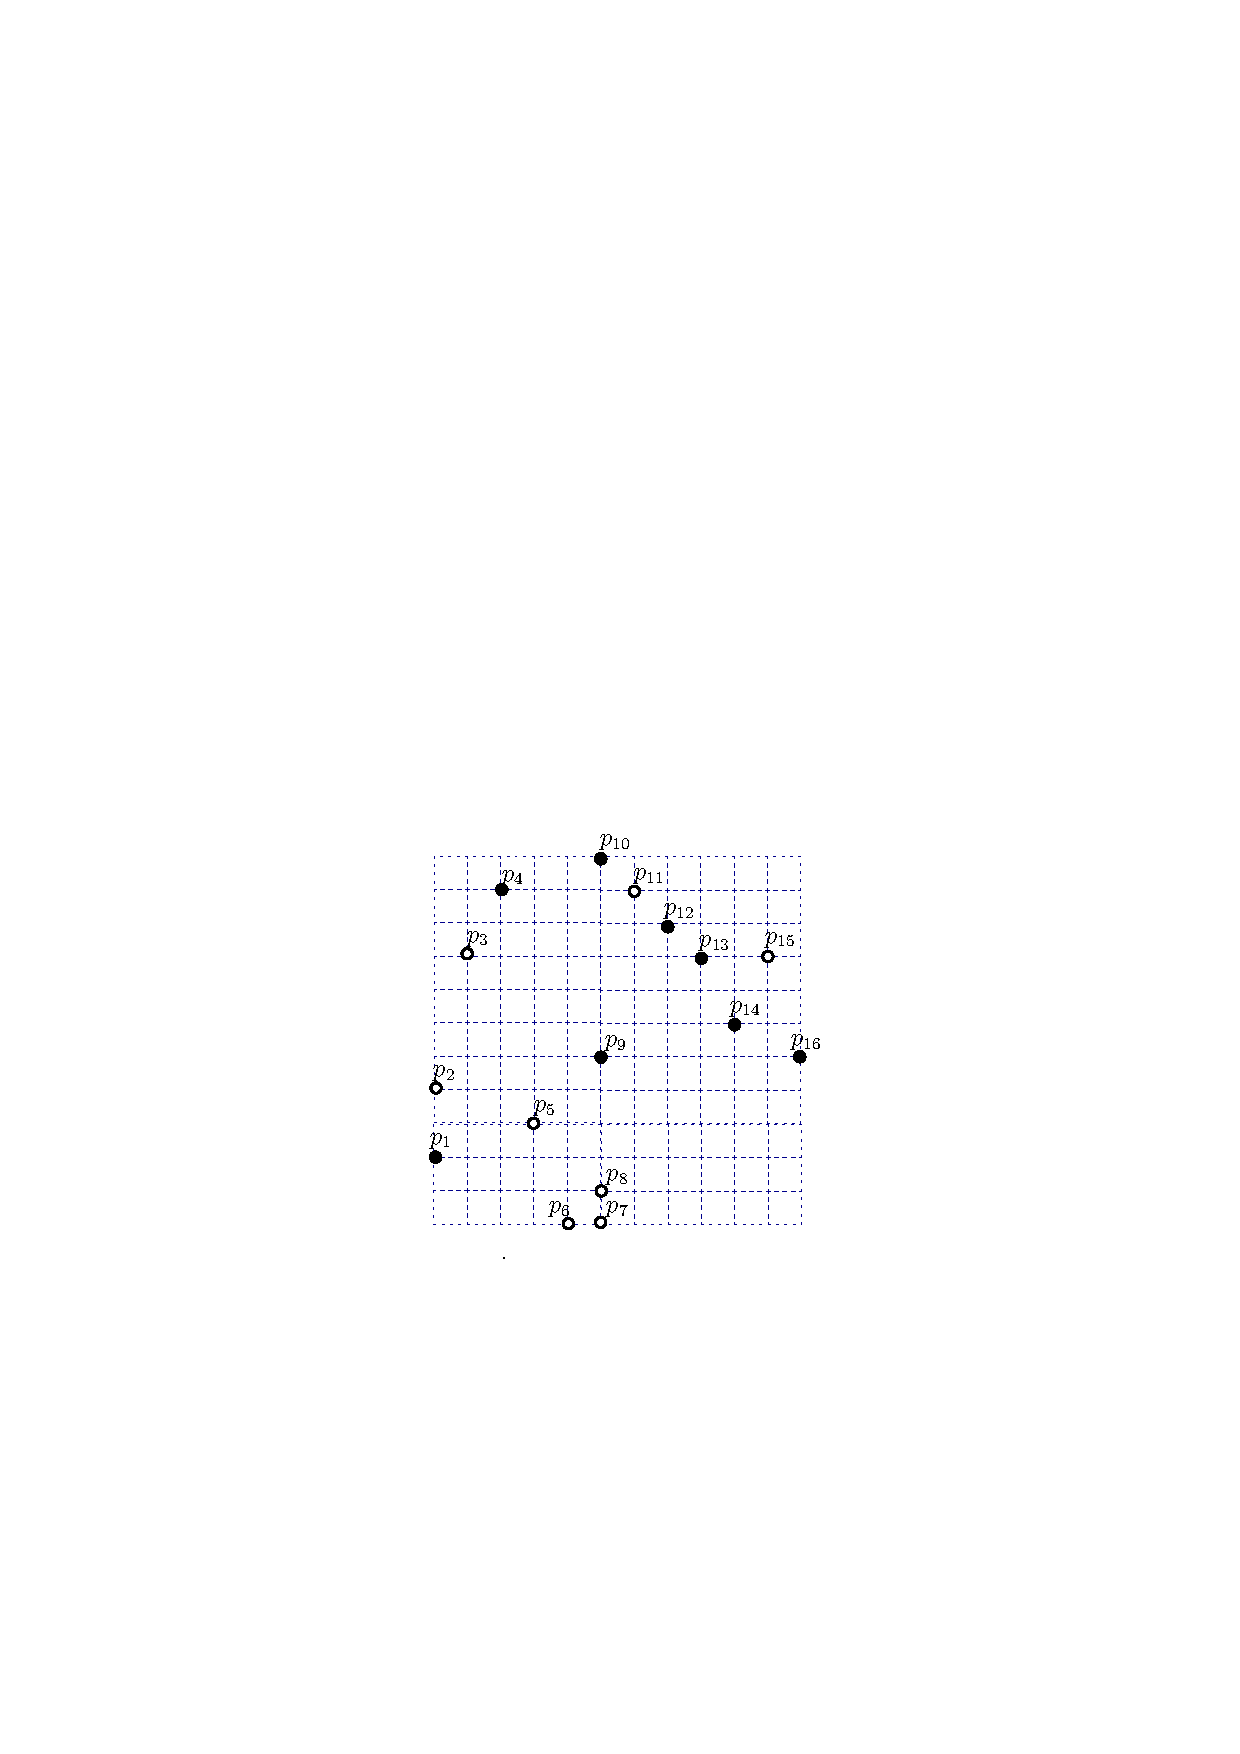
\includegraphics[height=40mm]{./artwork/ds} 
   \end{center}
   
%    At the beginning, all labels are hidden (but the coordinates are revealed). \\ 
%    \blue{Goal:} Predict the label of each point with as few mistakes as possible. \\ 
   
  
\end{small}
\end{frame}
%-------------------------------------------------------------
% \begin{frame}
% \begin{small}
%    
% %    In $\red{d}$-dimensional space, a point $\red{p}$ \blue{dominates} another point $\red{q}$ if $p[i] \ge q[i]$ for all $i \in [1, d]$. 
%    
%    \xmybox{Dominance} 
%    
%    \begin{center}
%        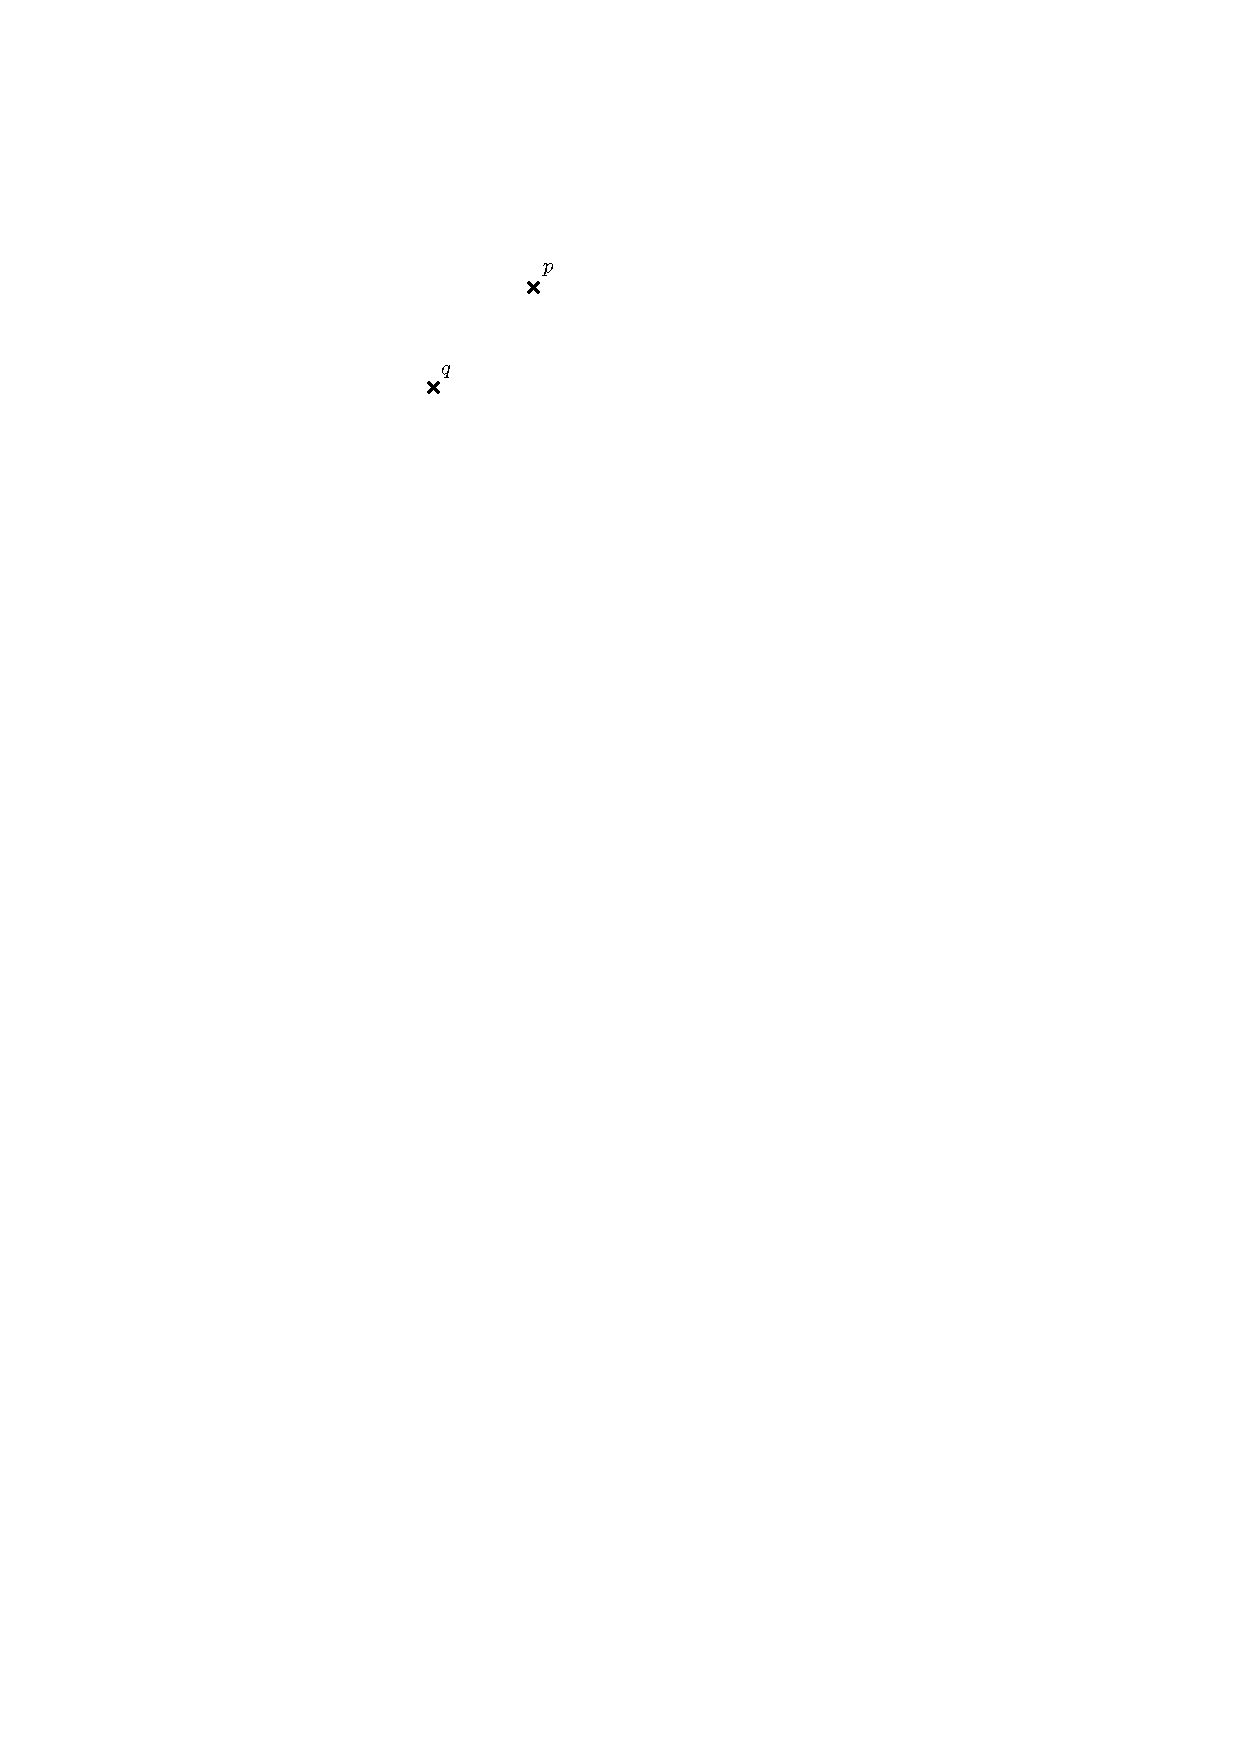
\includegraphics[height=17mm]{./artwork/dom} 
%    \end{center}
%    
%    \begin{center}
%        $p$ dominates $q$
%    \end{center}
% 
%   
% \end{small}
% \end{frame}
% %-------------------------------------------------------------
\myfrm{
    \xmybox{Monotone Classifier} 
    
    \begin{center}
       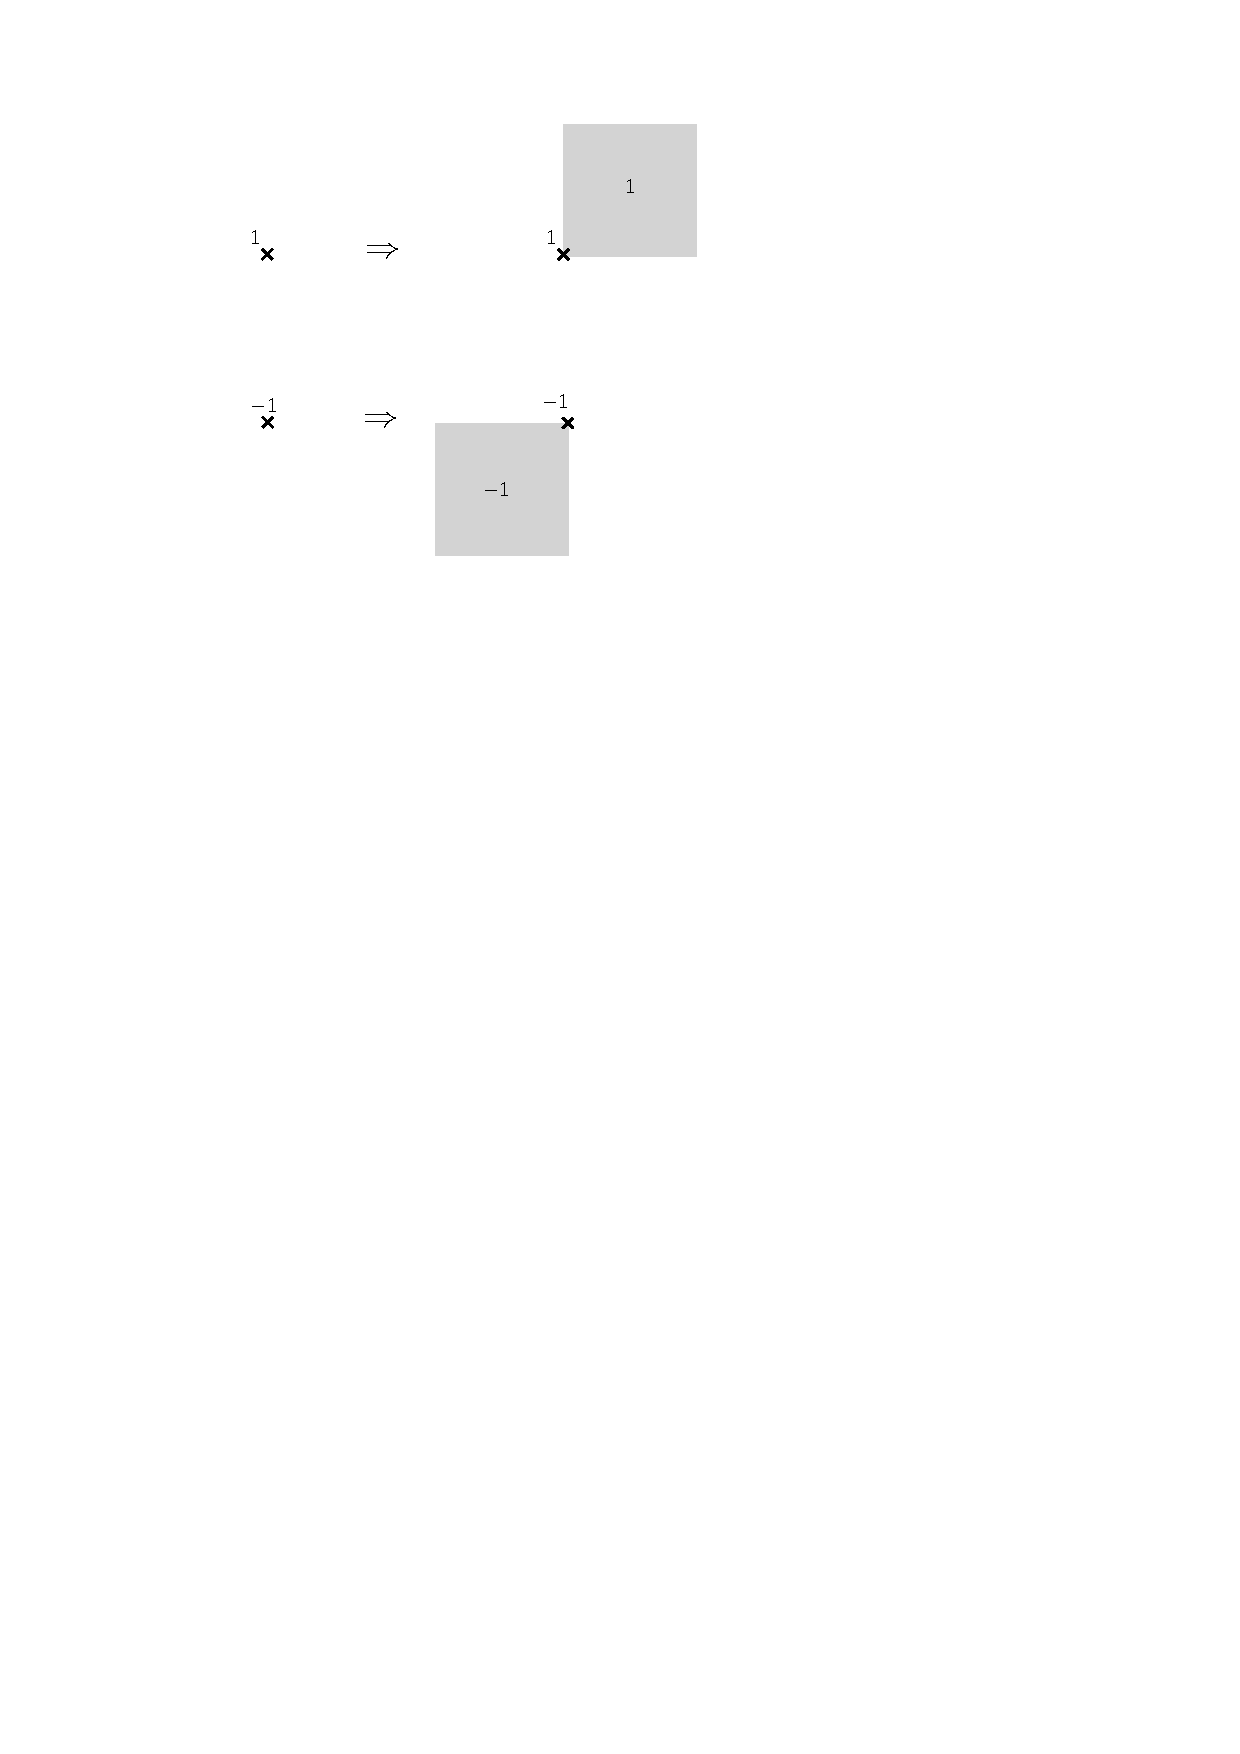
\includegraphics[height=50mm]{./artwork/dom-classifier} 
   \end{center}
}
%-------------------------------------------------------------
\myfrm{
    \xmybox{Monotone Classifier} 
    
    Examples:
    \begin{center}
       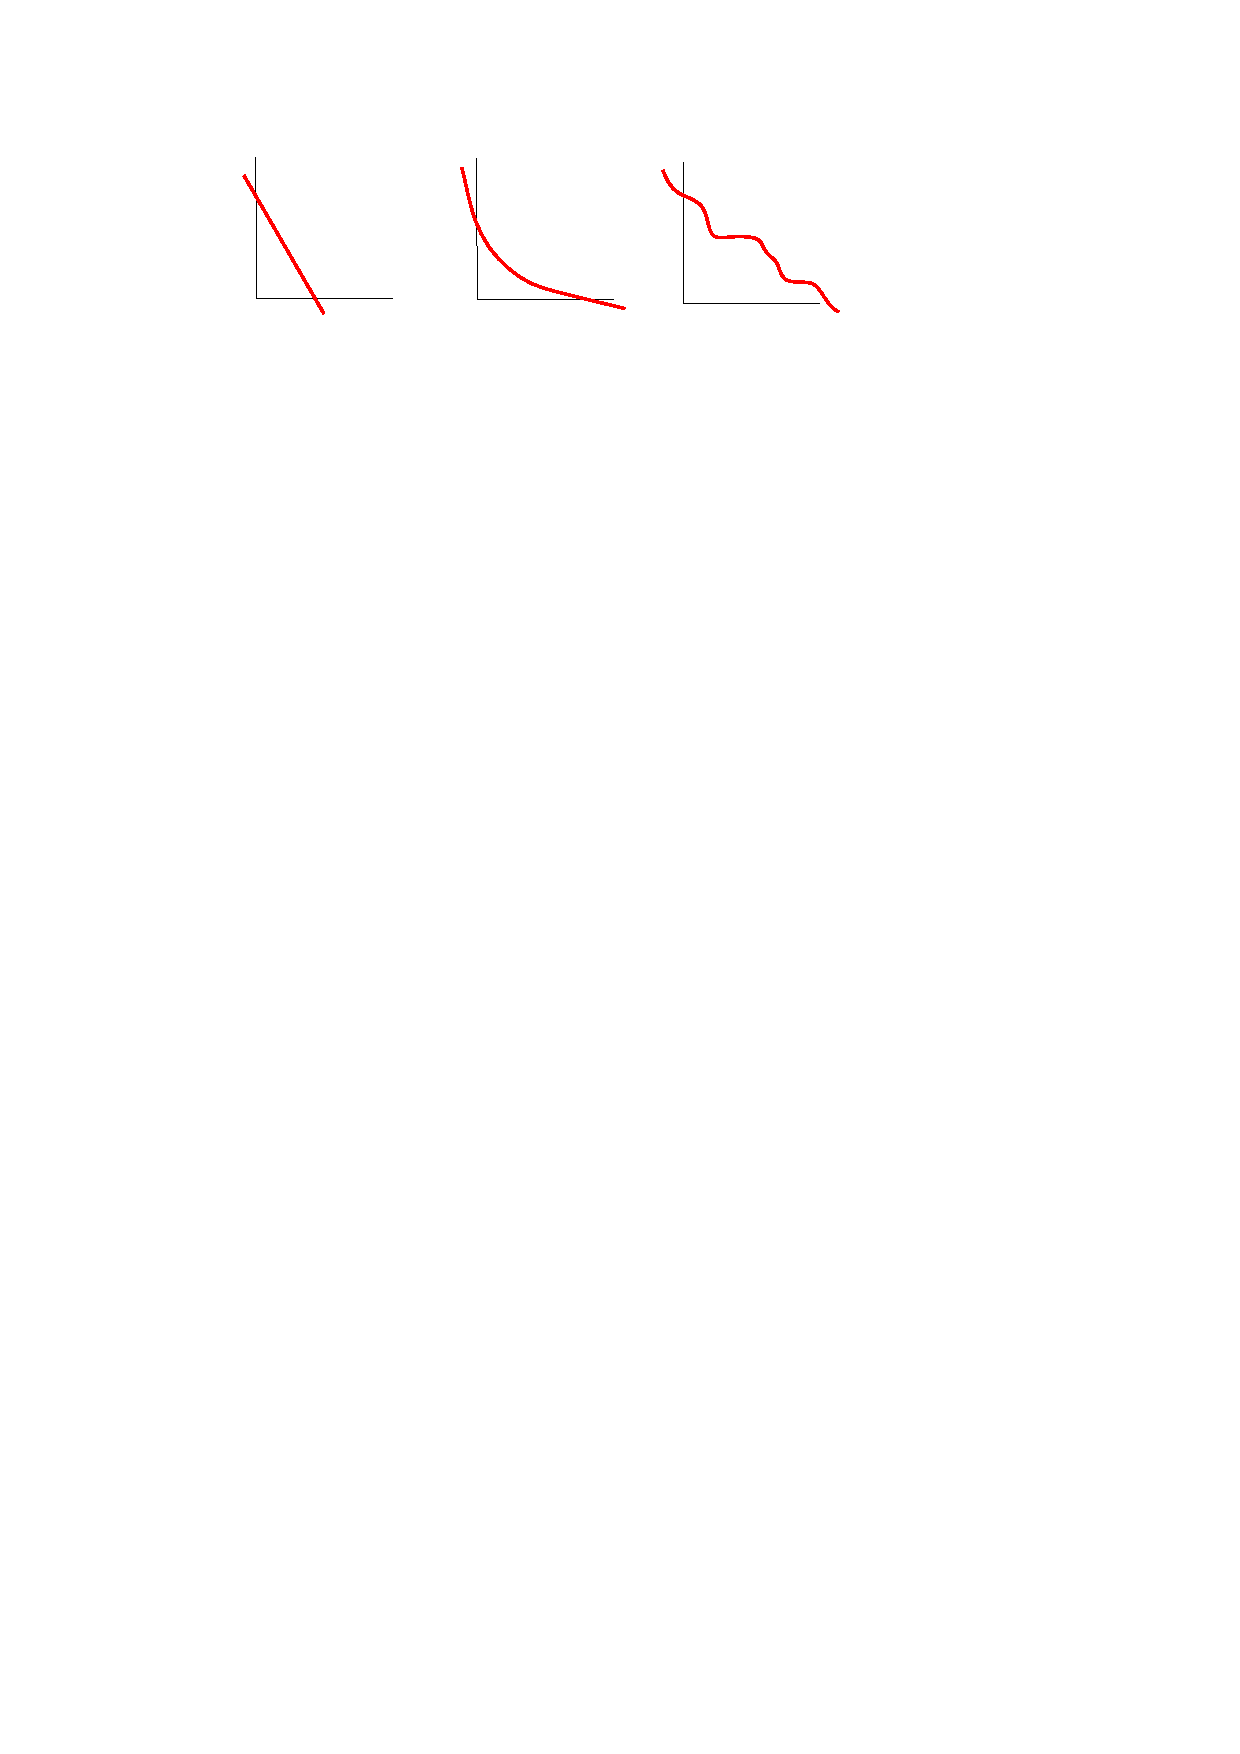
\includegraphics[height=25mm]{./artwork/dom-classifier-ex} 
   \end{center}
}
%-------------------------------------------------------------
\myfrm{

    \cbox{blue}{
    \centering
        $\red{k^*}$ = minimum error of all monotone classifiers 
    }
    
   \pause 
   
   \vgap
   
   \begin{center}
       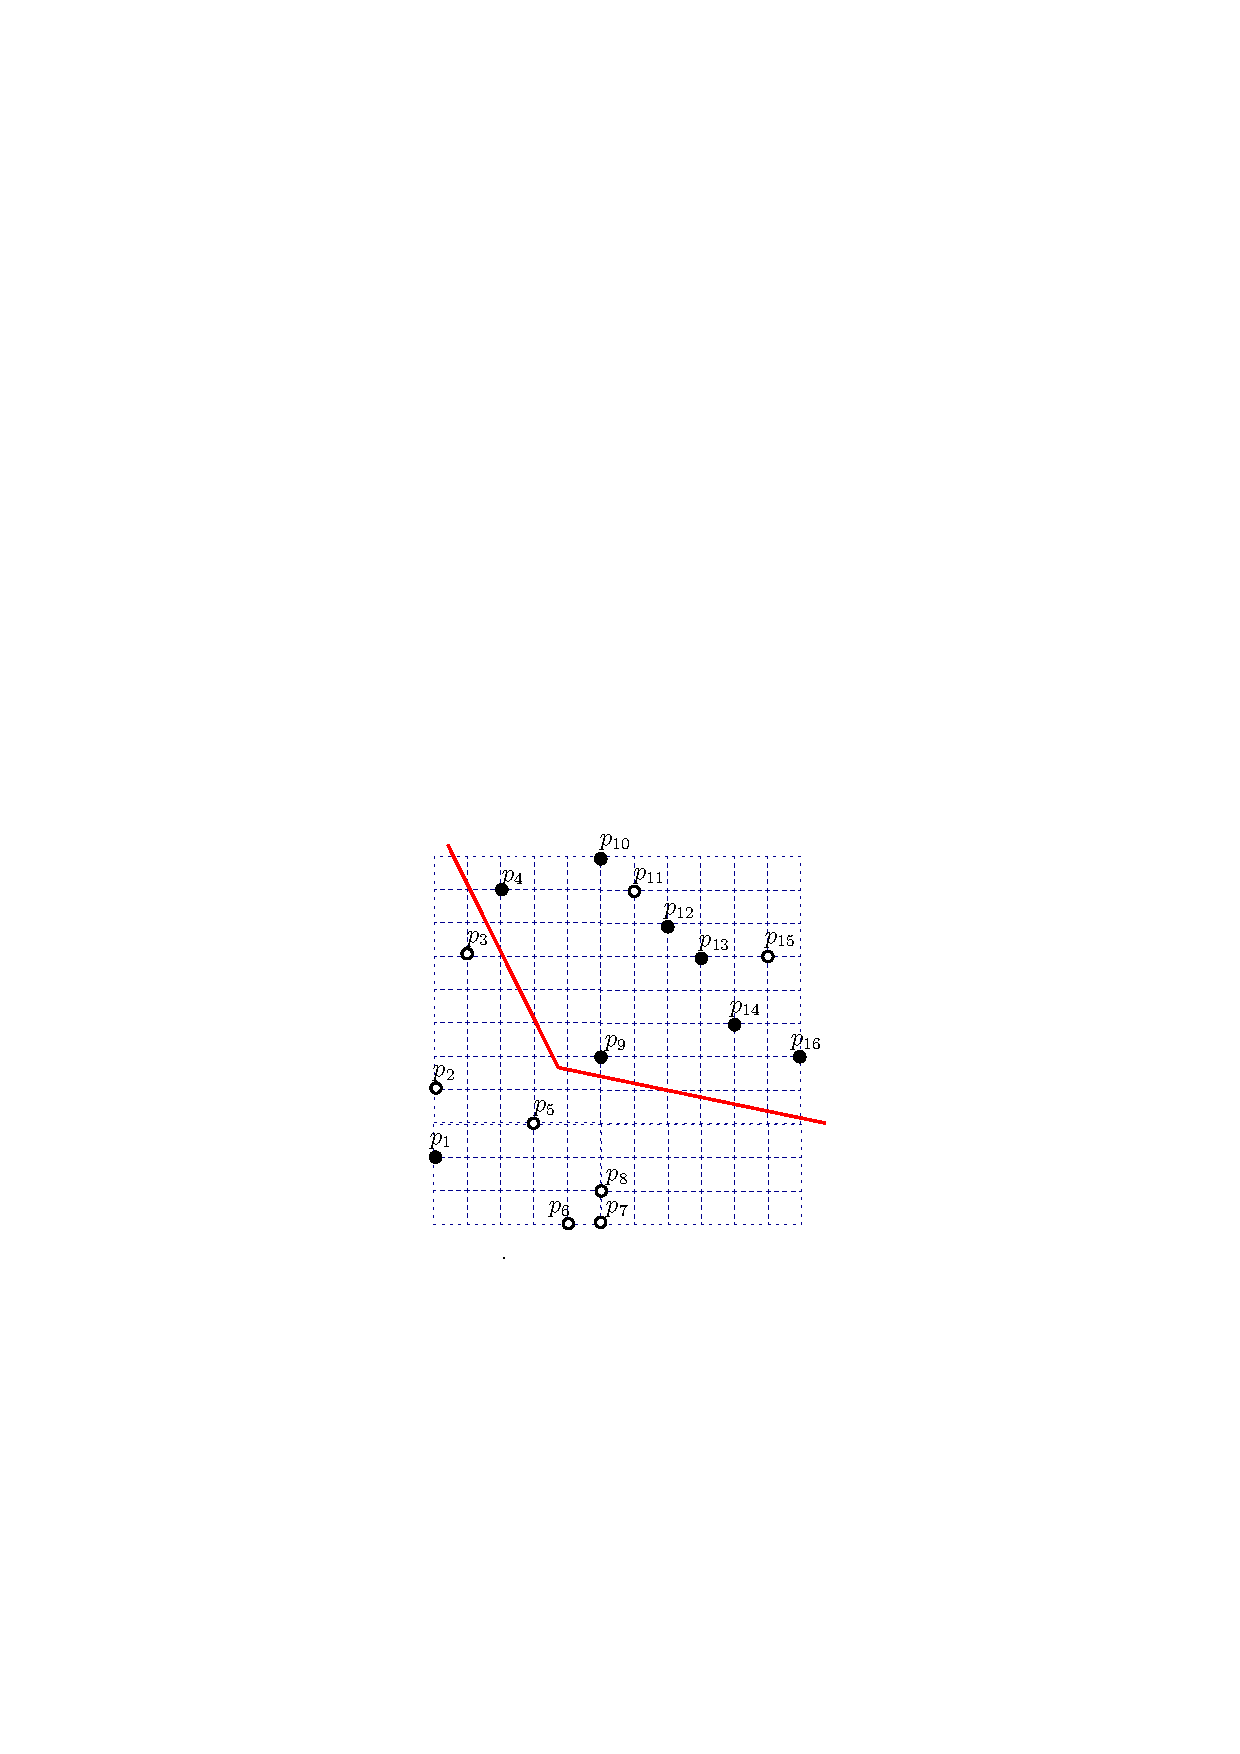
\includegraphics[height=40mm]{./artwork/ds-mono} 
       
       (black = 1, white = $-1$) \\[2mm]
       $k^* = 3$
   \end{center}
}
%-------------------------------------------------------------
\myfrm{
    \xmybox{Active Monotone Classification} 
    
    \vgap 
    
    \begin{center}
       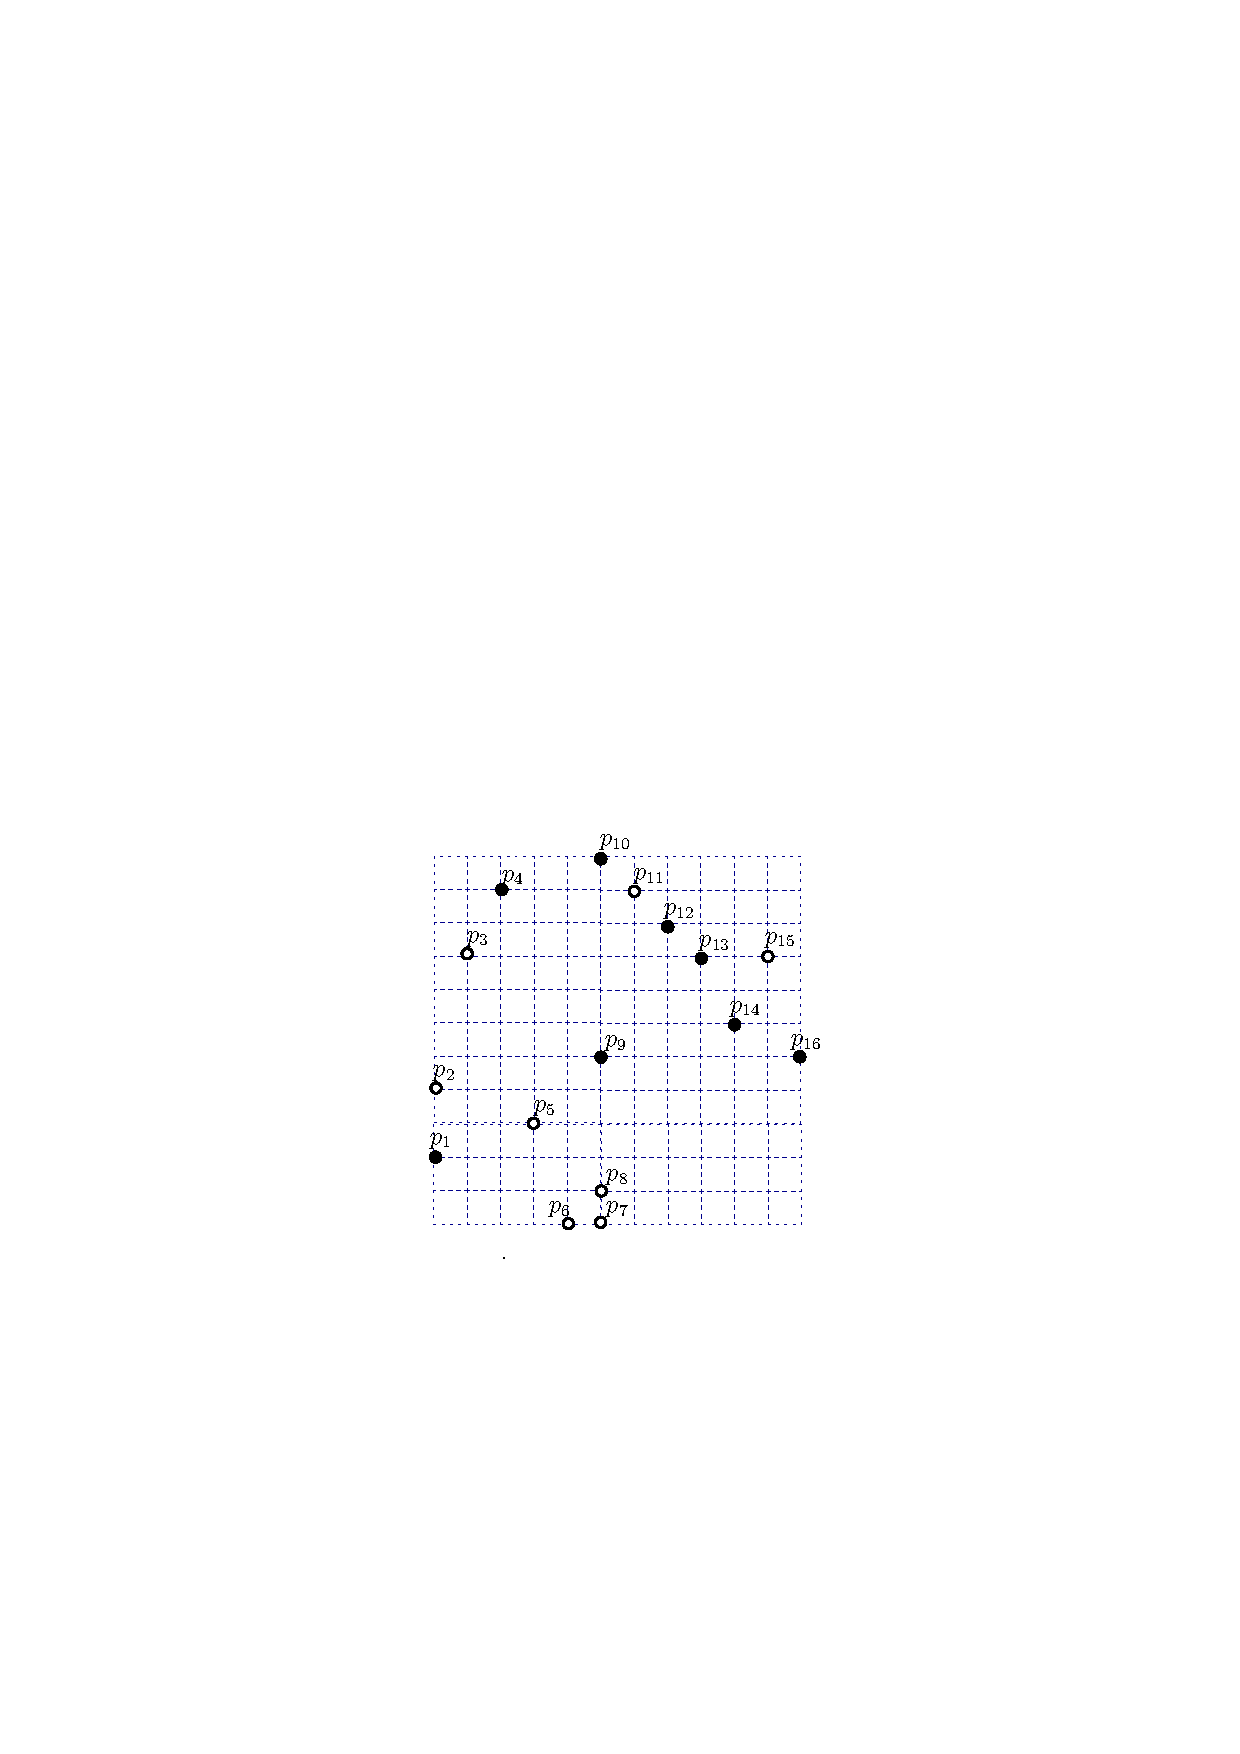
\includegraphics[height=40mm]{./artwork/ds} 
   \end{center}
   
   \vgap 
   
   \cbox{blue}{
   \blue{Question:} How many points must we probe to return a monotone classifier whose error is $k^*$? 
   }
}
%-------------------------------------------------------------
\myfrm{
    \blue{Dominance width} $\red{w}$ of $P$ 
    
     \begin{center}
       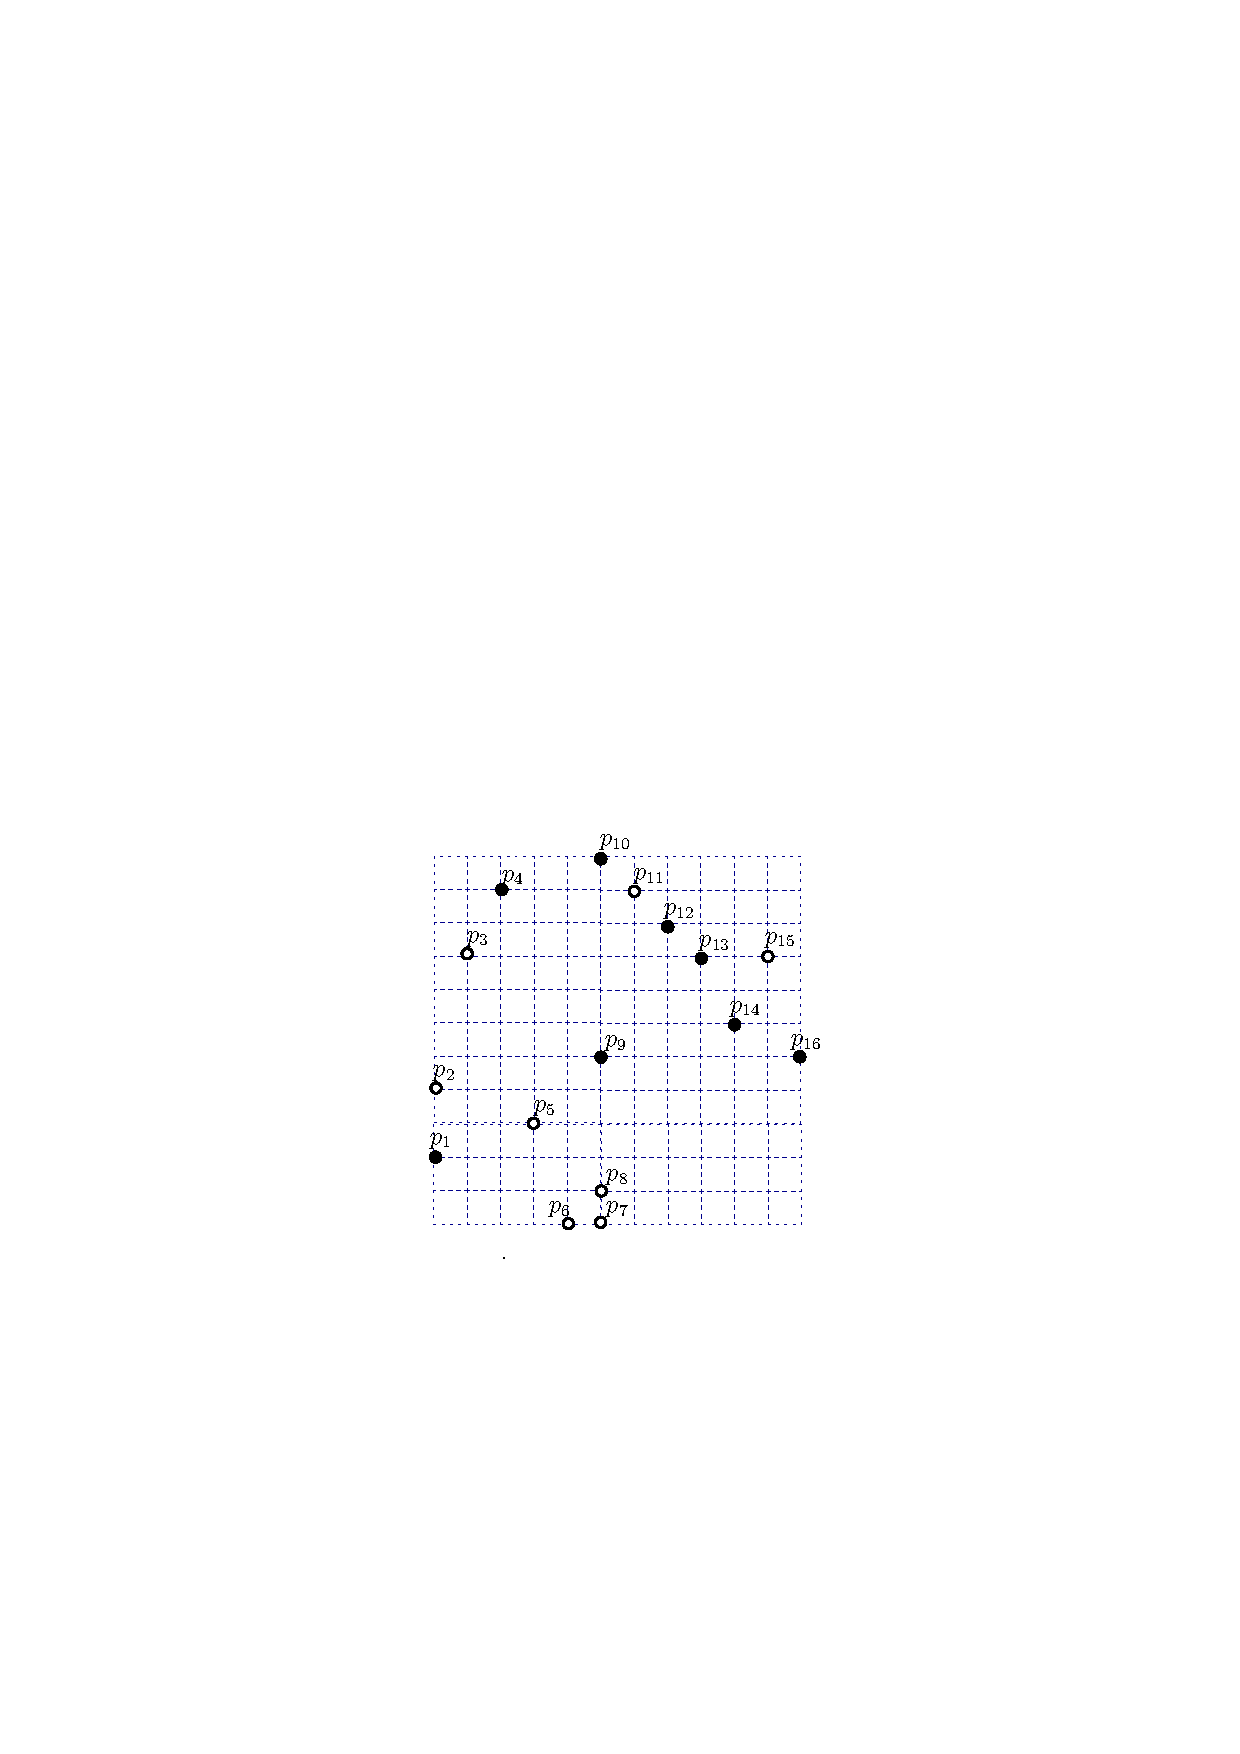
\includegraphics[height=40mm]{./artwork/ds} 
       
       $w$ = 6
   \end{center}
}
%-------------------------------------------------------------
\myfrm{
    \cbox{red}{
    \blue{Thm 1} [Tao and Wang'21]: \\
    $\Omega(n)$ to ensure error $k^*$, even in 1D. 
    }
    \pause
    
    \cbox{red}{
    \blue{Thm 2} [Tao'18]: \\
    $\Omega(w \log \fr{n}{(1+k^*) w})$ to ensure error $\red{c} k^*$, regardless of constant $c > 0$.
    }
    \pause 
    
    \cbox{green}{
    \blue{Thm 3} [Tao and Wang'21]: \\
    $O(w \log \fr{n}{w} \cdot \log n)$ to ensure error $(1+\eps) k^*$, for any constant $\eps > 0$. 
    }
    
    \pause 
    \cbox{green}{
    \blue{Thm 4} [Tao'18]: \\
    $O(w \log \fr{n}{w})$ (expected) probes to ensure (expected) $2 k^*$. 
    }
    
    
    
    
    %\blue{Remark:} For a long time, the best was $O(w^2)$ probes for $(1+\eps) k^*$. 
}
%-------------------------------------------------------------
\begin{frame}{} 
\begin{small}
    \xmybox{2-Approximate Algorithm}
    
    \begin{center} 
        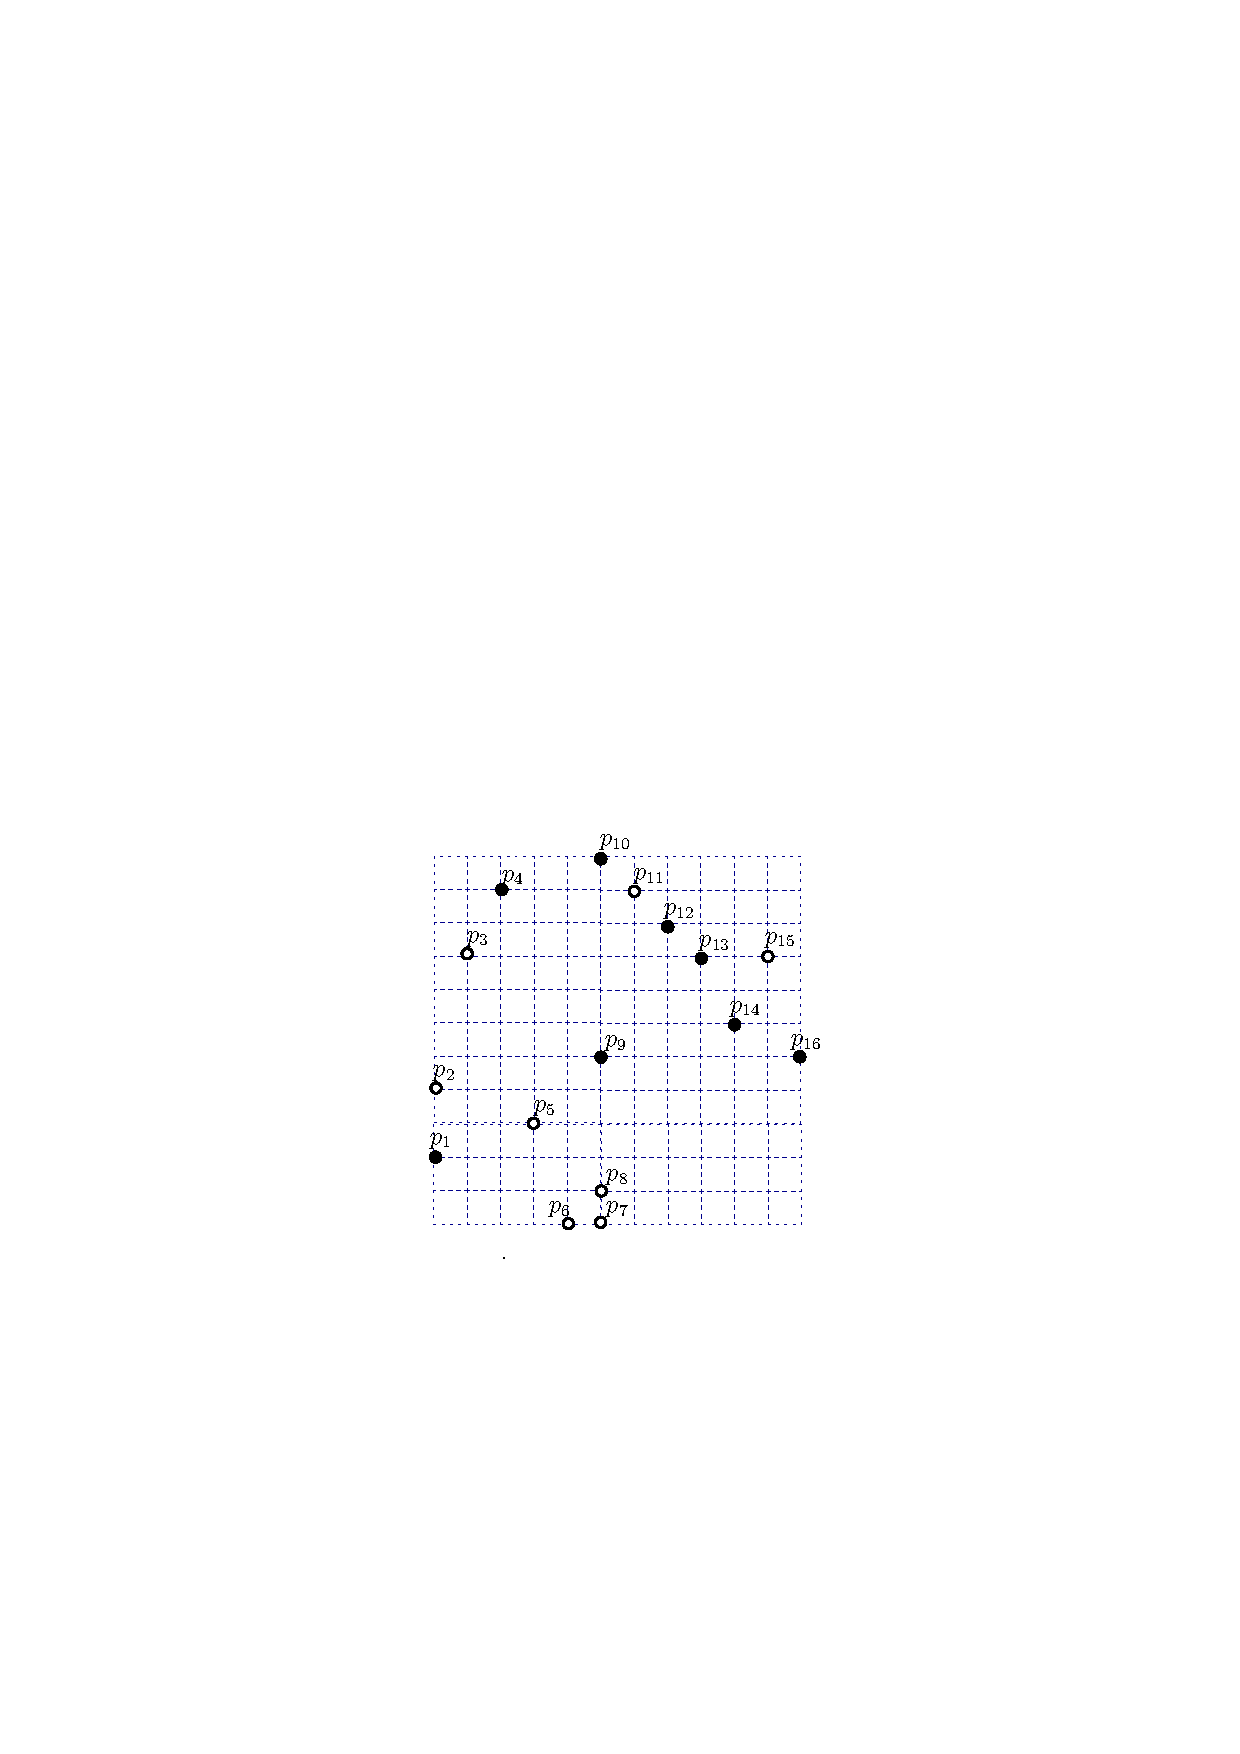
\includegraphics[height=40mm]{./artwork/ds} \\ 
    \end{center}
    
    \pause 
    First probe = $p_1$ \\ 
    \pause 
    Second = $p_8$ \\
    \pause 
    Returns a classifier with error 5

\end{small}
\end{frame}
%-------------------------------------------------------------
\begin{frame}{} 
\begin{small}
    \begin{center} 
         \mybox[yellow]{II: Crowdsourcing}
    \end{center}
\end{small}
\end{frame}
%-------------------------------------------------------------
\begin{frame}{}
\begin{small}
    \xmybox{Partial Order Search}  
    
    \begin{center} 
         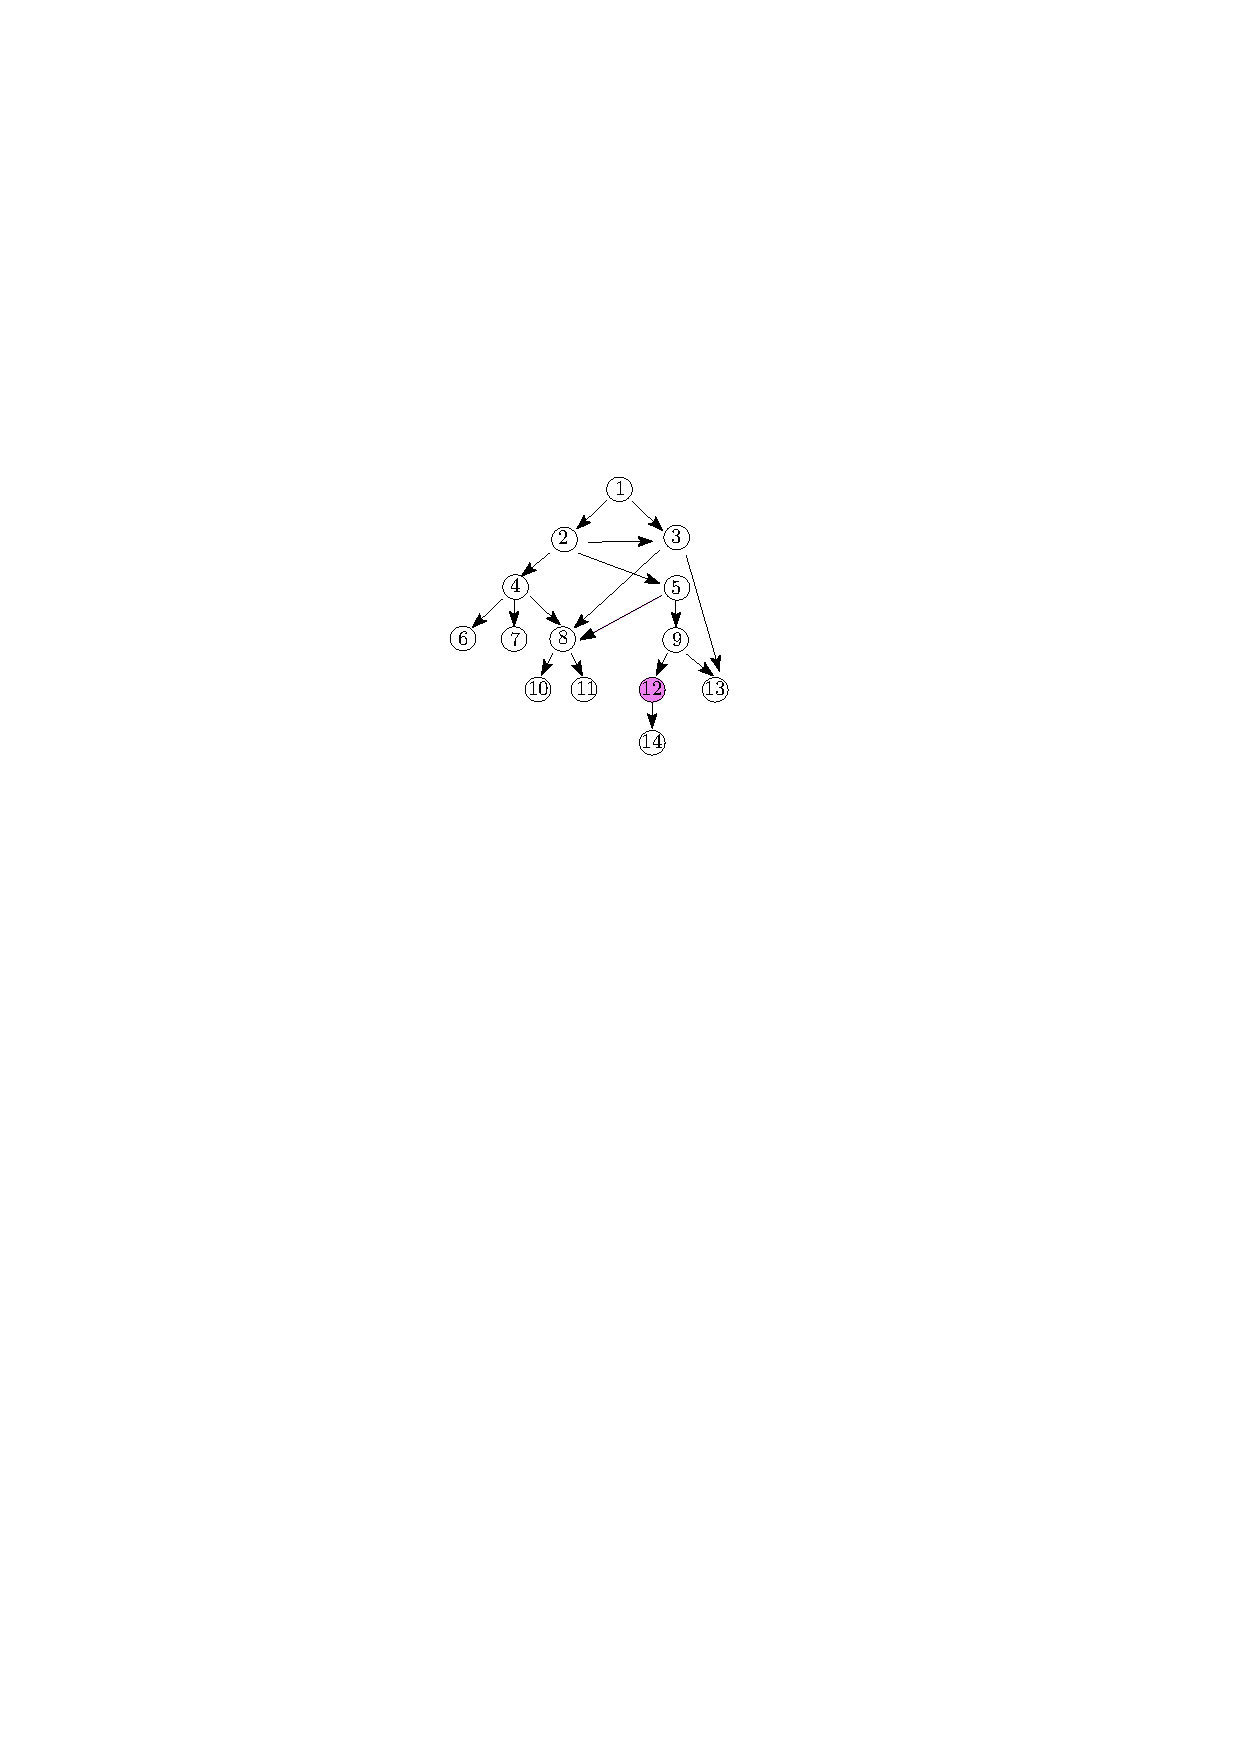
\includegraphics[height=40mm]{./artwork/running-dag1}
    \end{center}


\end{small}
\end{frame}
%-------------------------------------------------------------
\begin{frame}{}
\begin{small}
    \xmybox{Crowdsourcing}
    
    \vgap\vgap 
    
     \begin{center}
         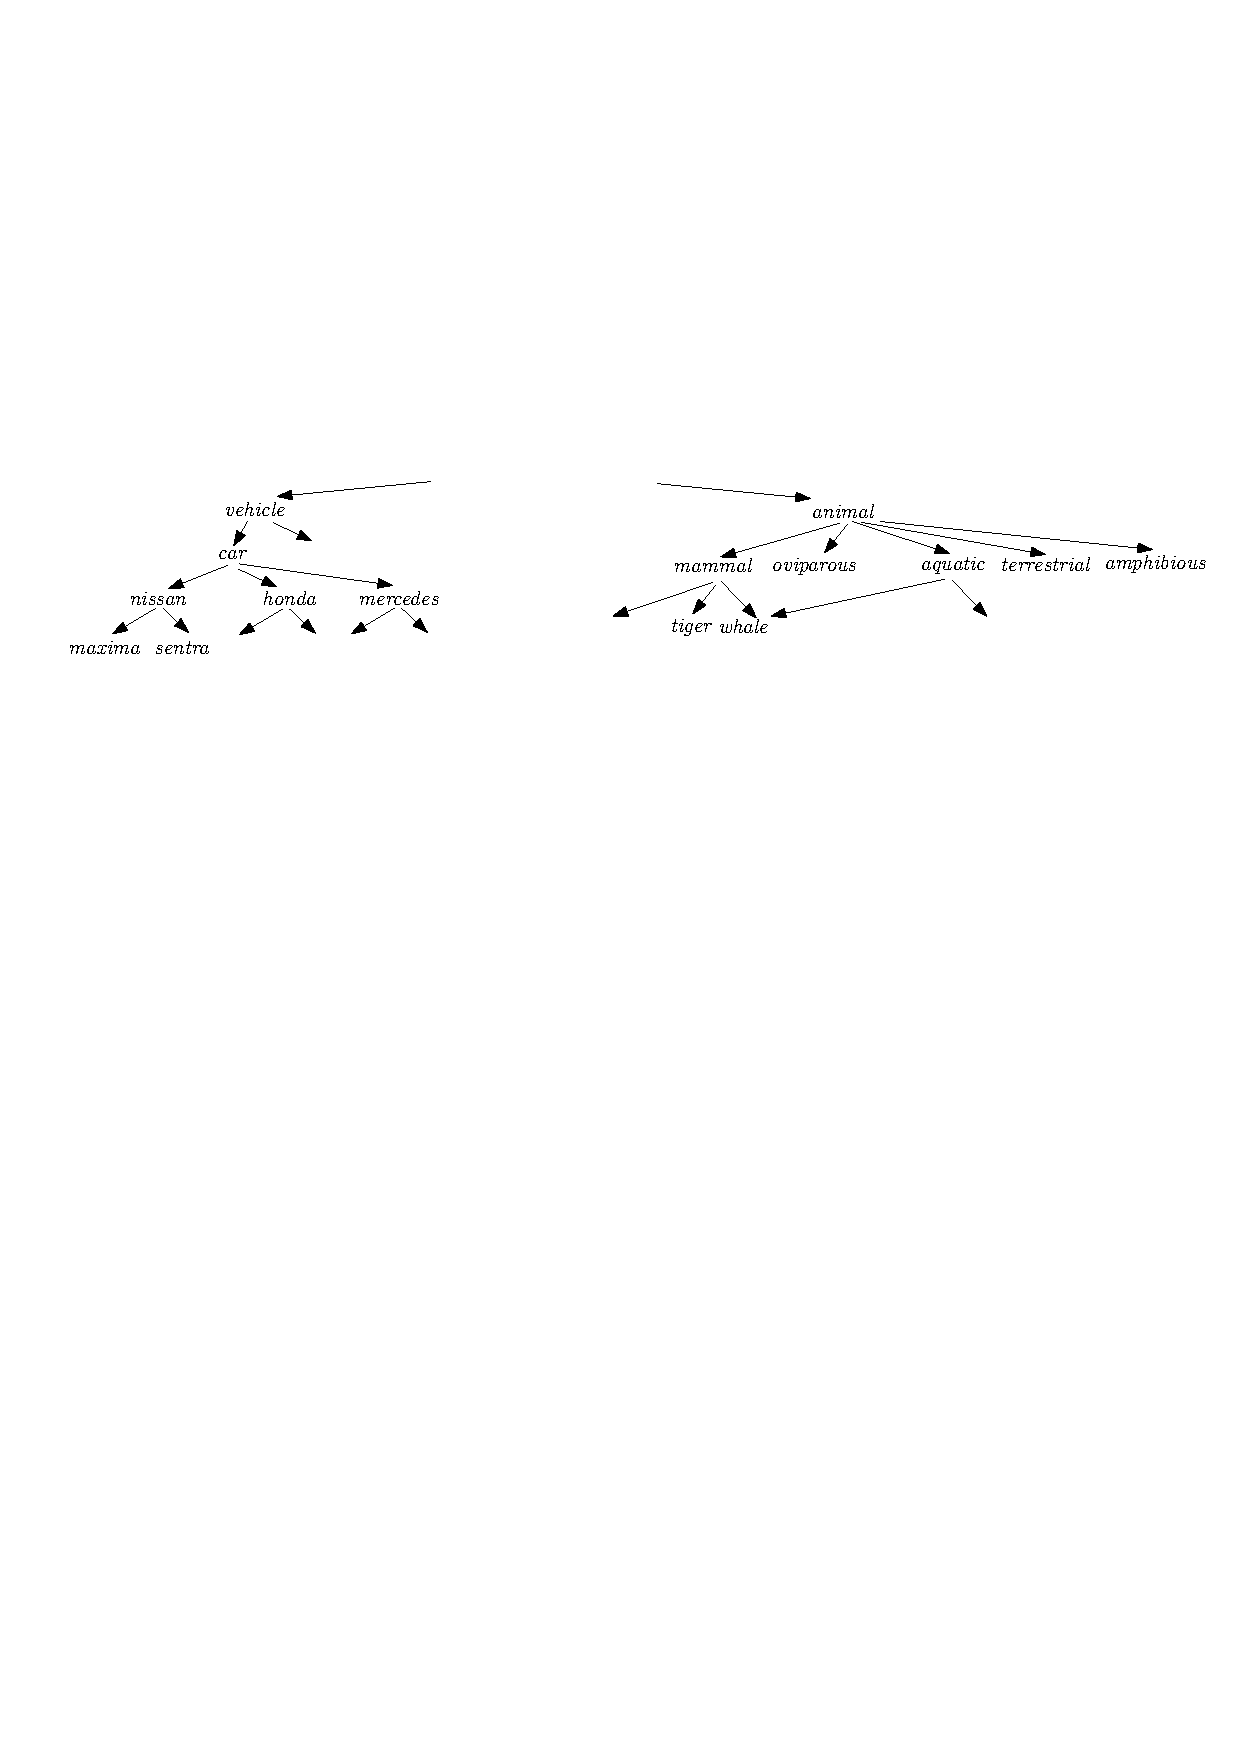
\includegraphics[width=\linewidth]{./artwork/intro-hier} 
    \end{center}

    
    \begin{center} 
         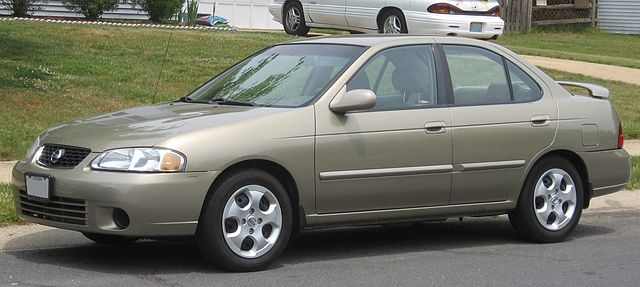
\includegraphics[height=23mm]{./artwork/sentra.jpg} 
         \hspace{10mm}
         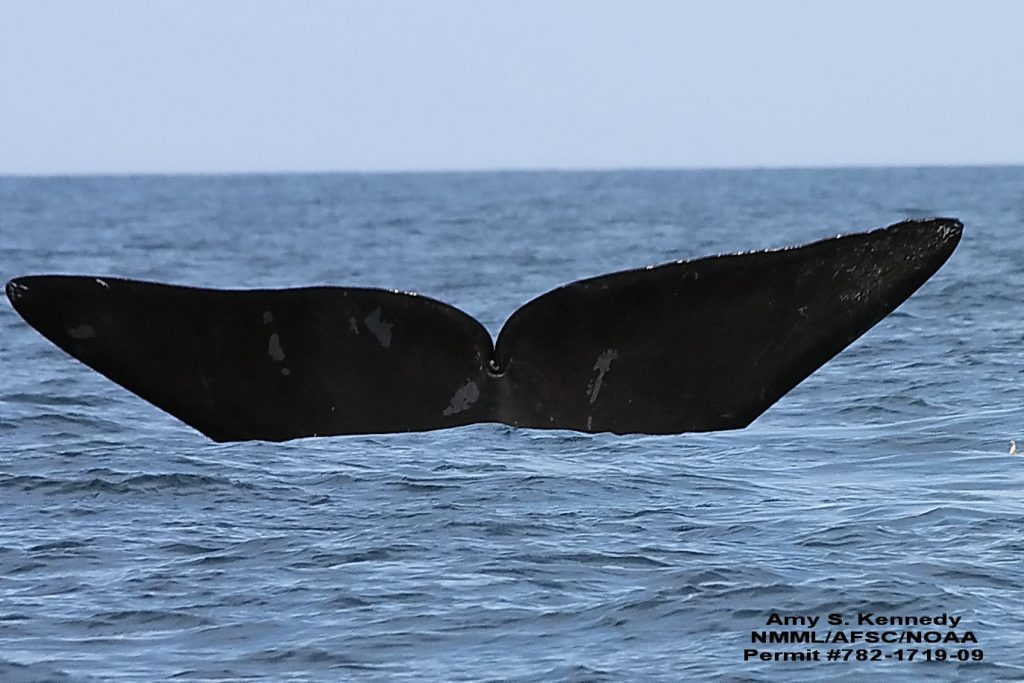
\includegraphics[height=23mm]{./artwork/whale.jpg} 
    \end{center}

    
\end{small}
\end{frame}
%-------------------------------------------------------------
\myfrm{
    $\red{n} =$ number of nodes \\
    $\red{d} =$ maximum out-degree \\
    $\red{k} =$ number of questions in each round \\
    
    \vgap
    
    \cbox{red}{
    \blue{Thm 1} [Lu, Martens, Niewerth, Tao'21] \\ 
    $\Omega(\log_{1+k} n + \fr{d}{k} \log_{1+d} n)$ probes necessary. 
   }
   
   \vgap
    
    \cbox{green}{
    \blue{Thm 2} [Lu, Martens, Niewerth, Tao'21] \\ 
    $O(\log_{1+k} n + \fr{d}{k} \log_{1+d} n)$ probes suffice. 
   }
}
%-------------------------------------------------------------
\myfrm{
    With roughly $1 + d/k$ probes, we can achieve: 
    \begin{center}
        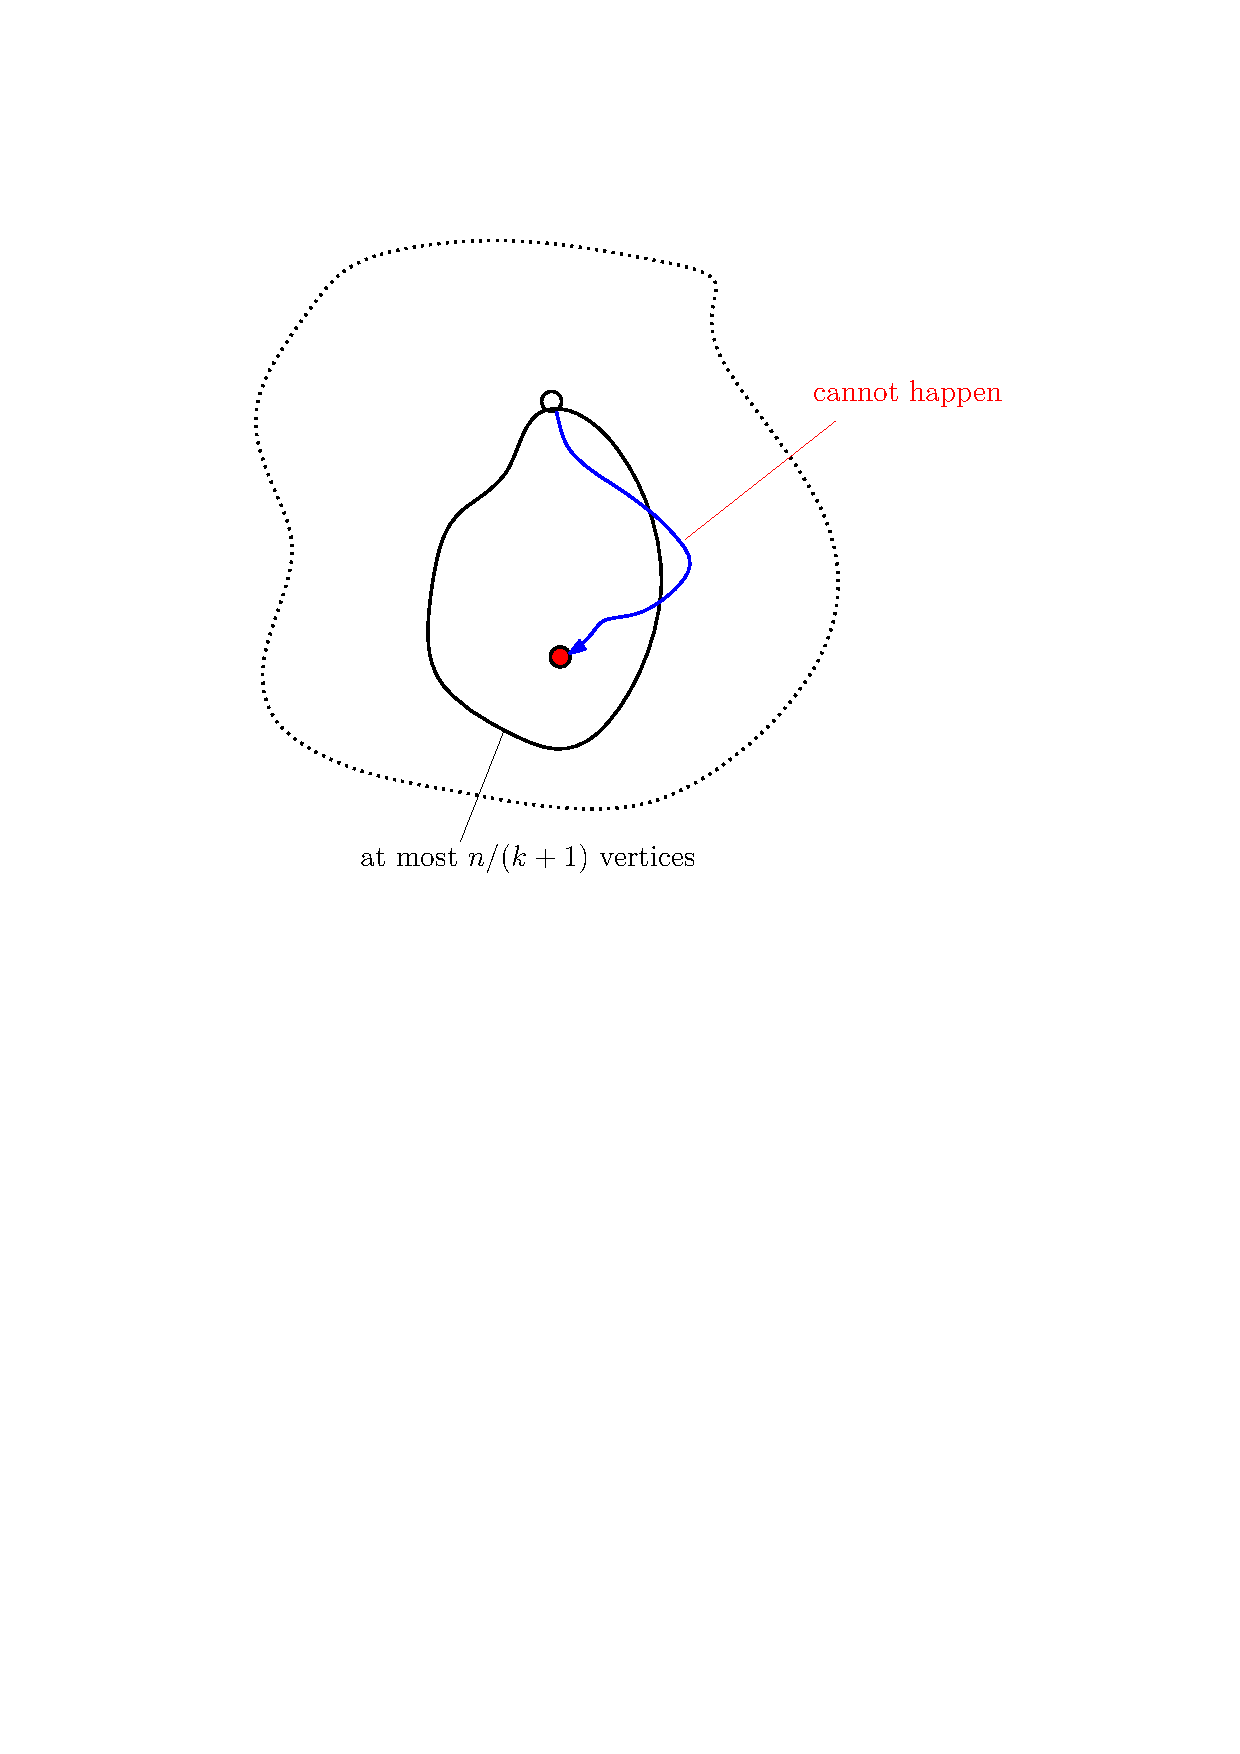
\includegraphics[height=60mm]{./artwork/poms-idea}
    \end{center}
}
%-------------------------------------------------------------
\begin{frame}{} 
\begin{small}
    \begin{center} 
         \mybox[yellow]{III: Massively Parallel Computation}
    \end{center}
\end{small}
\end{frame}
%-------------------------------------------------------------
\myfrm{
    \xmybox{Subgraph Enumeration}
    
    \vgap\vgap
    
    \begin{center}
        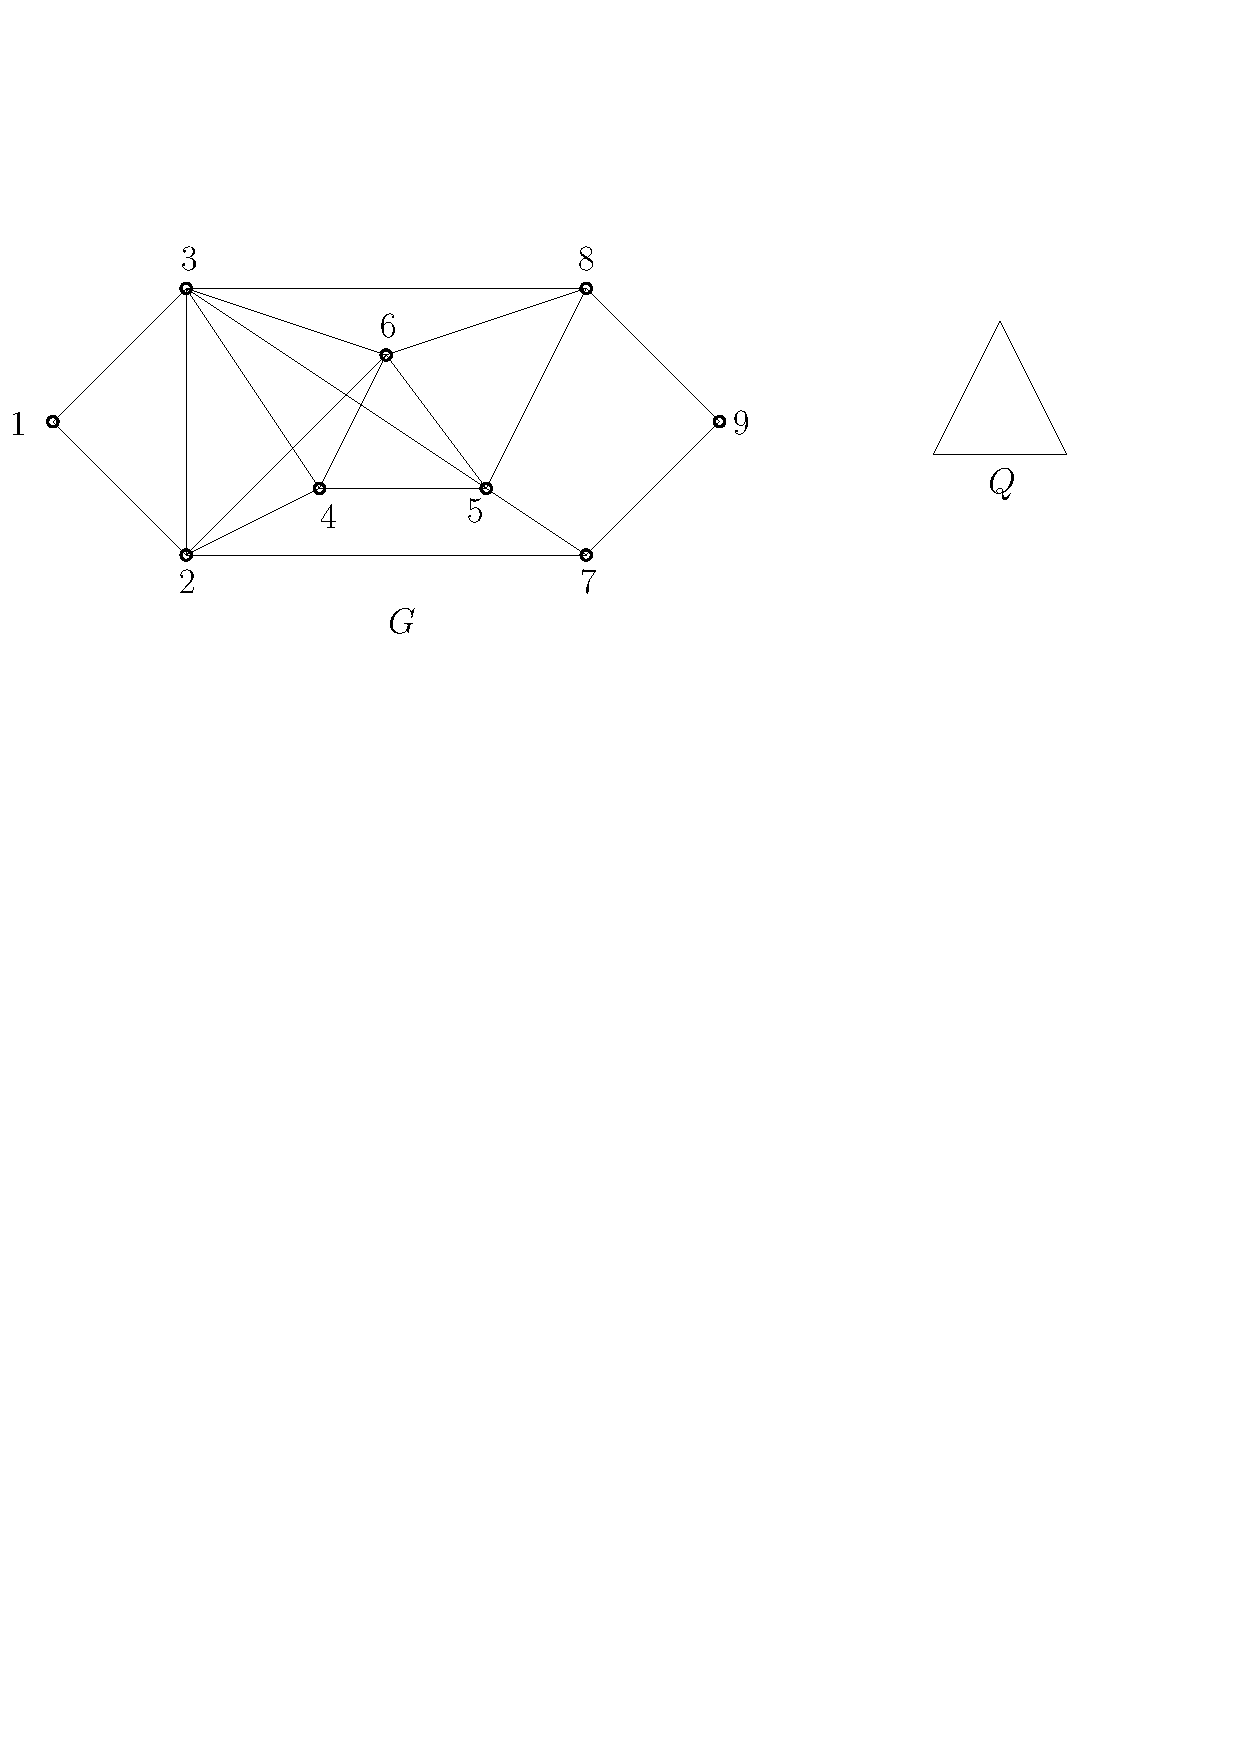
\includegraphics[height=32mm]{./artwork/subgraph-ex1}
    \end{center}
}
%-------------------------------------------------------------
\myfrm{ 
    \xmybox{MPC} 
    
    \vgap\vgap
    \begin{center}
        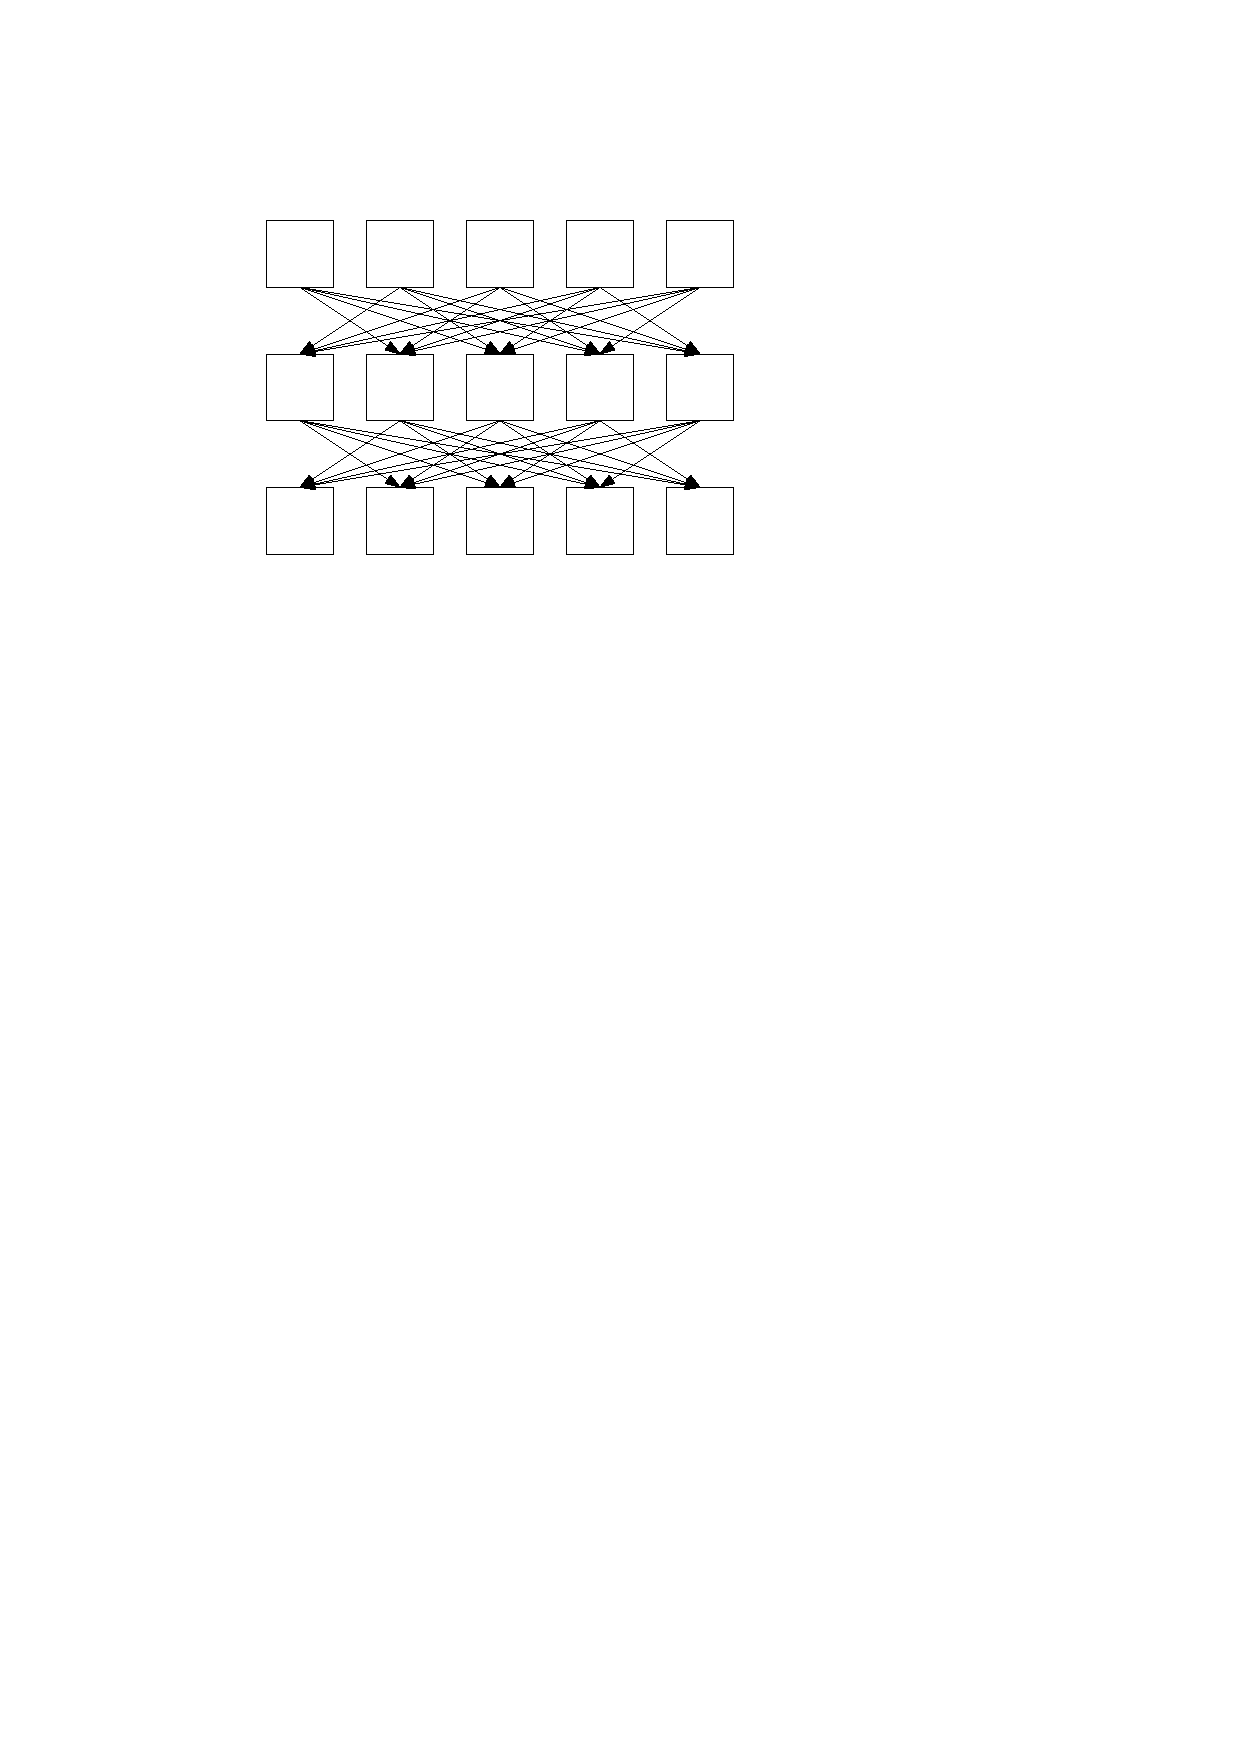
\includegraphics[height=40mm]{./artwork/mpc}
    \end{center}
    
    \vgap
    \blue{Goal:} Minimize the amount of communication on every machine. 
}
%-------------------------------------------------------------
\myfrm{
    \xmybox{AGM Bound}
    
    \vgap\vgap
    
    \begin{center}
        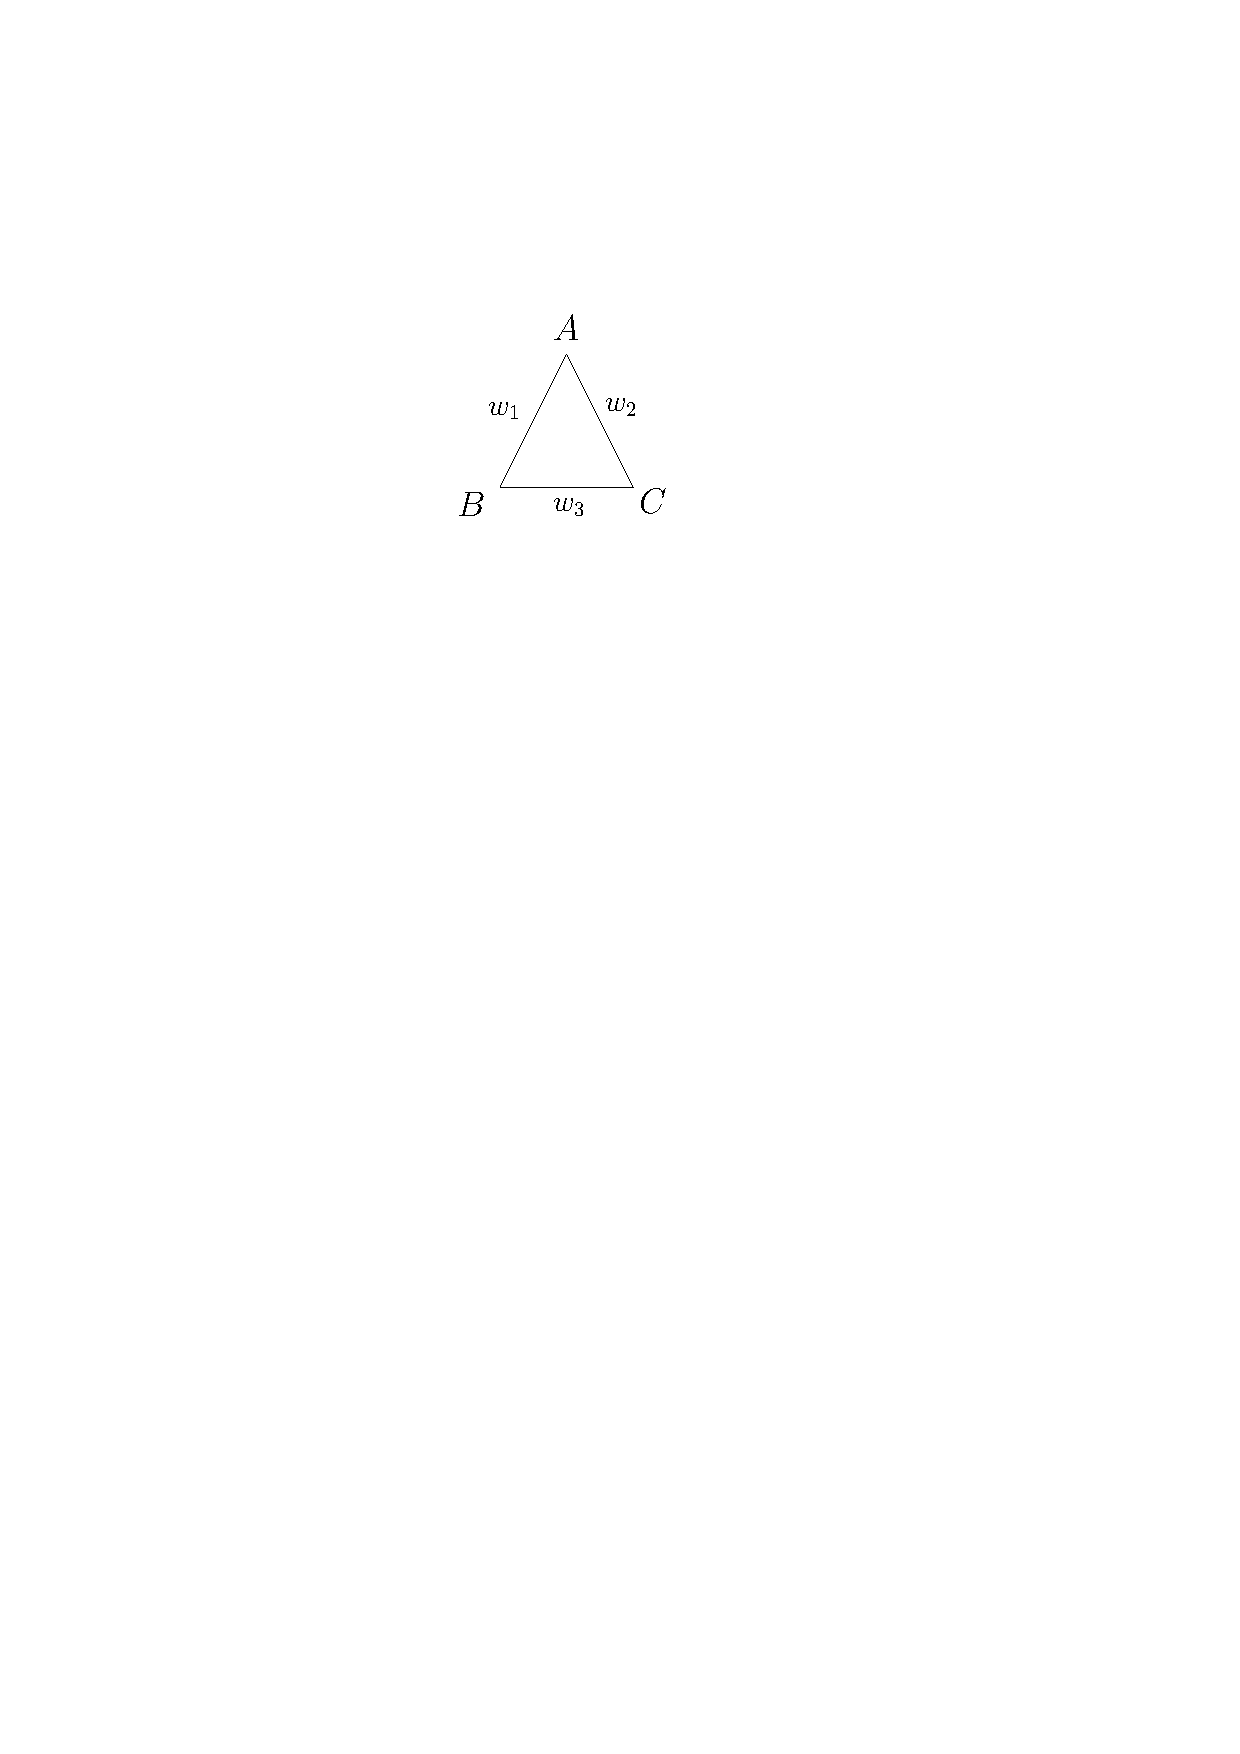
\includegraphics[height=18mm]{./artwork/agm}
    \end{center}
    
    Minimize $w_1 + w_2 + w_3$ subject to
    \myeqn{
        w_1 + w_2 \ge 1 \nn \\ 
        w_1 + w_3 \ge 1 \nn \\
        w_2 + w_3 \ge 1 \nn
    }
    
    \pause 
    
    Answer: 1.5 --- the \blue{fractional edge covering number} $\red{\rho}$ 
}
%-------------------------------------------------------------
\myfrm{
    \xmybox{AGM Bound}
    
    \vgap\vgap
    
    \begin{center}
        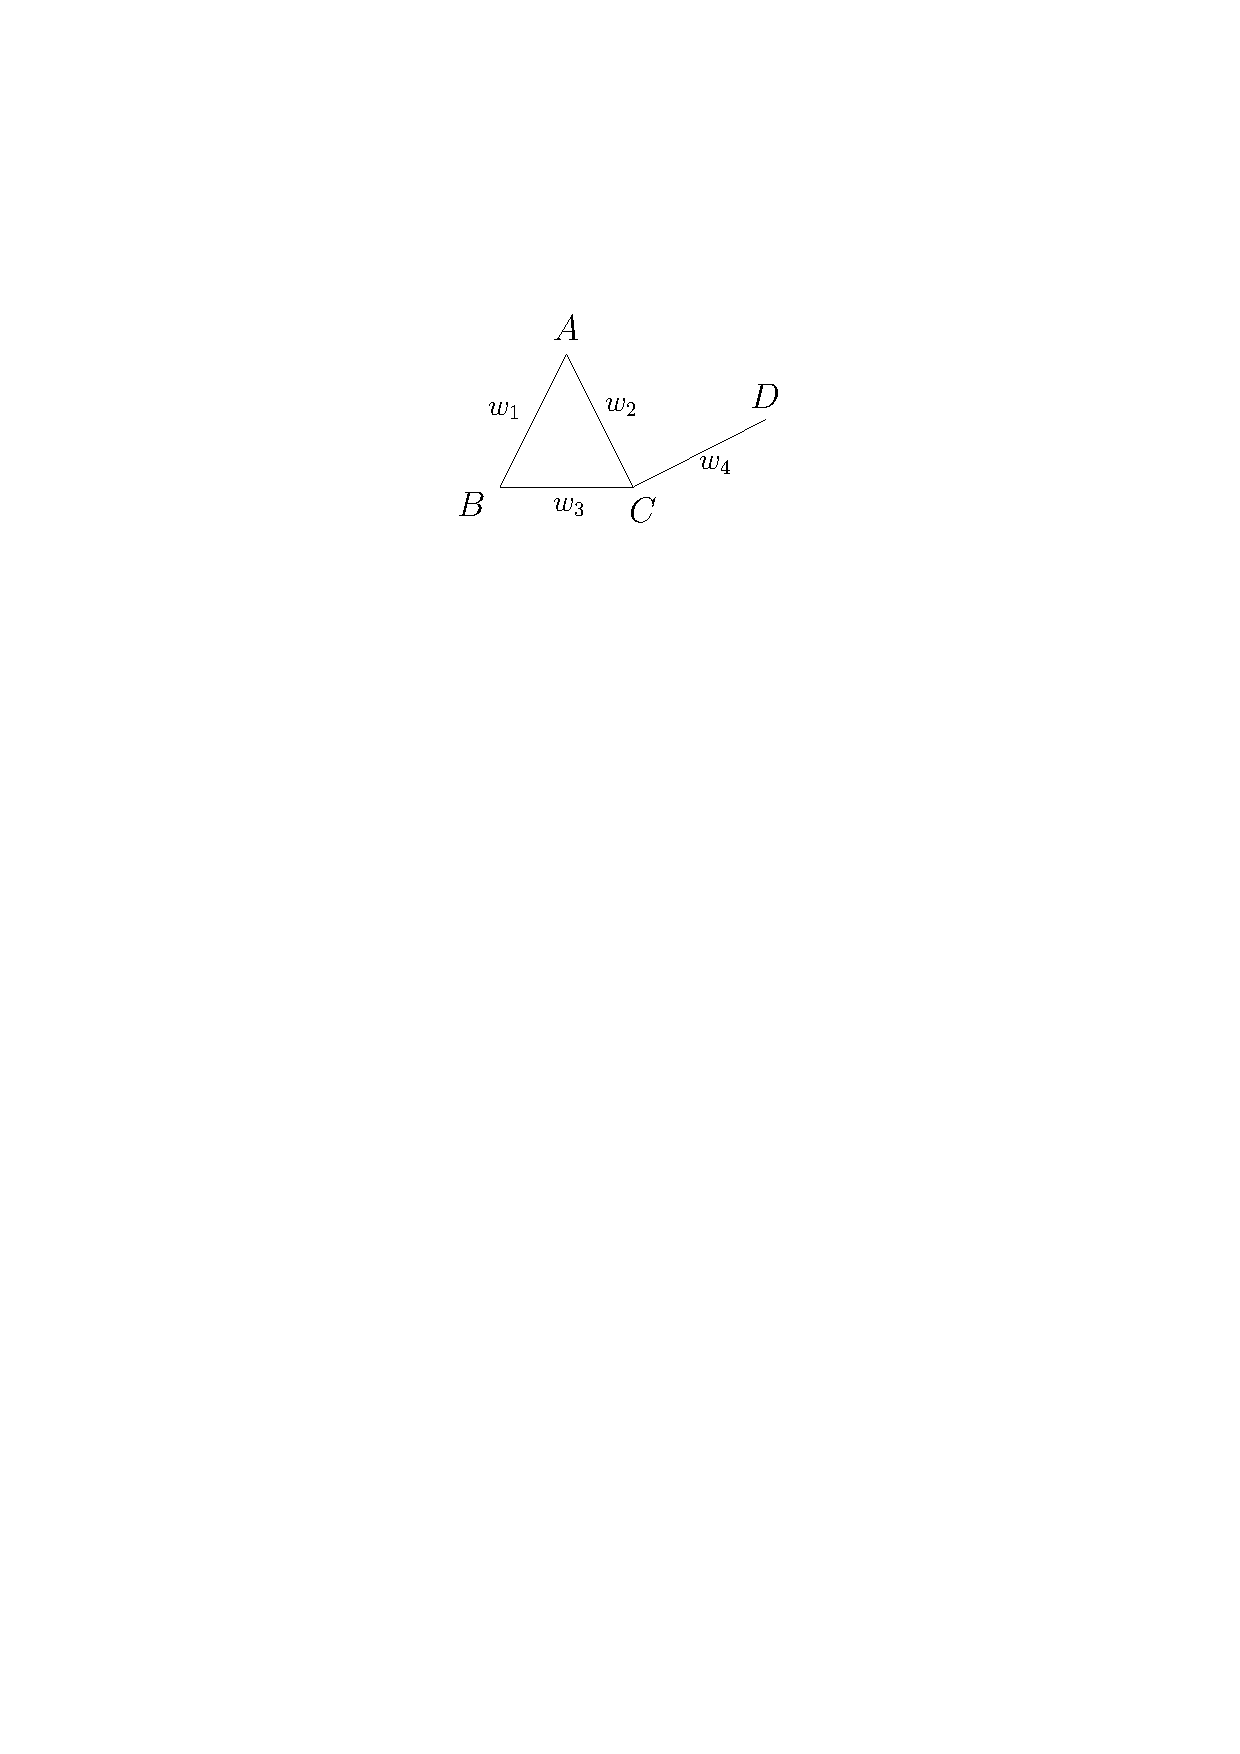
\includegraphics[height=18mm]{./artwork/agm2}
    \end{center}
    
    Minimize $w_1 + w_2 + w_3 + w_4$ subject to
    \myeqn{
        w_1 + w_2 &\ge& 1 \nn \\ 
        w_1 + w_3 &\ge& 1 \nn \\
        w_2 + w_3 + w_4 &\ge& 1 \nn \\
        w_4 &\ge& 1 \nn
    }
    
    \pause
    
    Answer: 2 --- the \blue{fractional edge covering number} $\red{\rho}$ 
}
%-------------------------------------------------------------
\myfrm{
    \xmybox{AGM Bound}
    
    \vgap\vgap
    \cbox{blue}{
        The maximum number of occurrences of $Q$ in a graph of $m$ edges is $\red{\Theta}(m^\rho)$.
    }
}
%-------------------------------------------------------------
\myfrm{
    %\xmybox{Lower Bound}

    $\red{p}$ = number of machines \\ 
    
    
    \cbox{red}{
        \blue{Thm 1} At least one machine must communicate $\Omega(m / p^{1/\rho})$. 
    }
    
    \vgap 
    
    \pause 
    Every machine sees at most $\red{L}$ edges  \\ \pause 
    $\Rightarrow$ Each machine can generate $O(L^\rho)$ occurrences of $Q$ \\ \pause 
    $\Rightarrow$ In total, $O(p \cdot L^\rho)$ occurrences \\  \pause 
    But in the worst case $G$ has $\Omega(m^\rho)$ occurrences of $Q$ \pause 
    \myeqn{
        \Rightarrow p \cdot L^\rho &=& \Omega(m^\rho) \nn
    }
    
    \pause 
    
    \cbox{green}{
        \blue{Thm 2} [Kestman, Suciu, Tao'20] \\
        $\tO(m / p^{1/\rho})$ communication per machine suffices. 
    }
}
%-------------------------------------------------------------
\myfrm{
    \begin{center} 
         \mybox[yellow]{IV: Dynamic Graphs}
    \end{center}
}
%-------------------------------------------------------------
\myfrm{
    \xmybox{Triangle Counting}
\vgap\vgap
    
    \begin{center}
        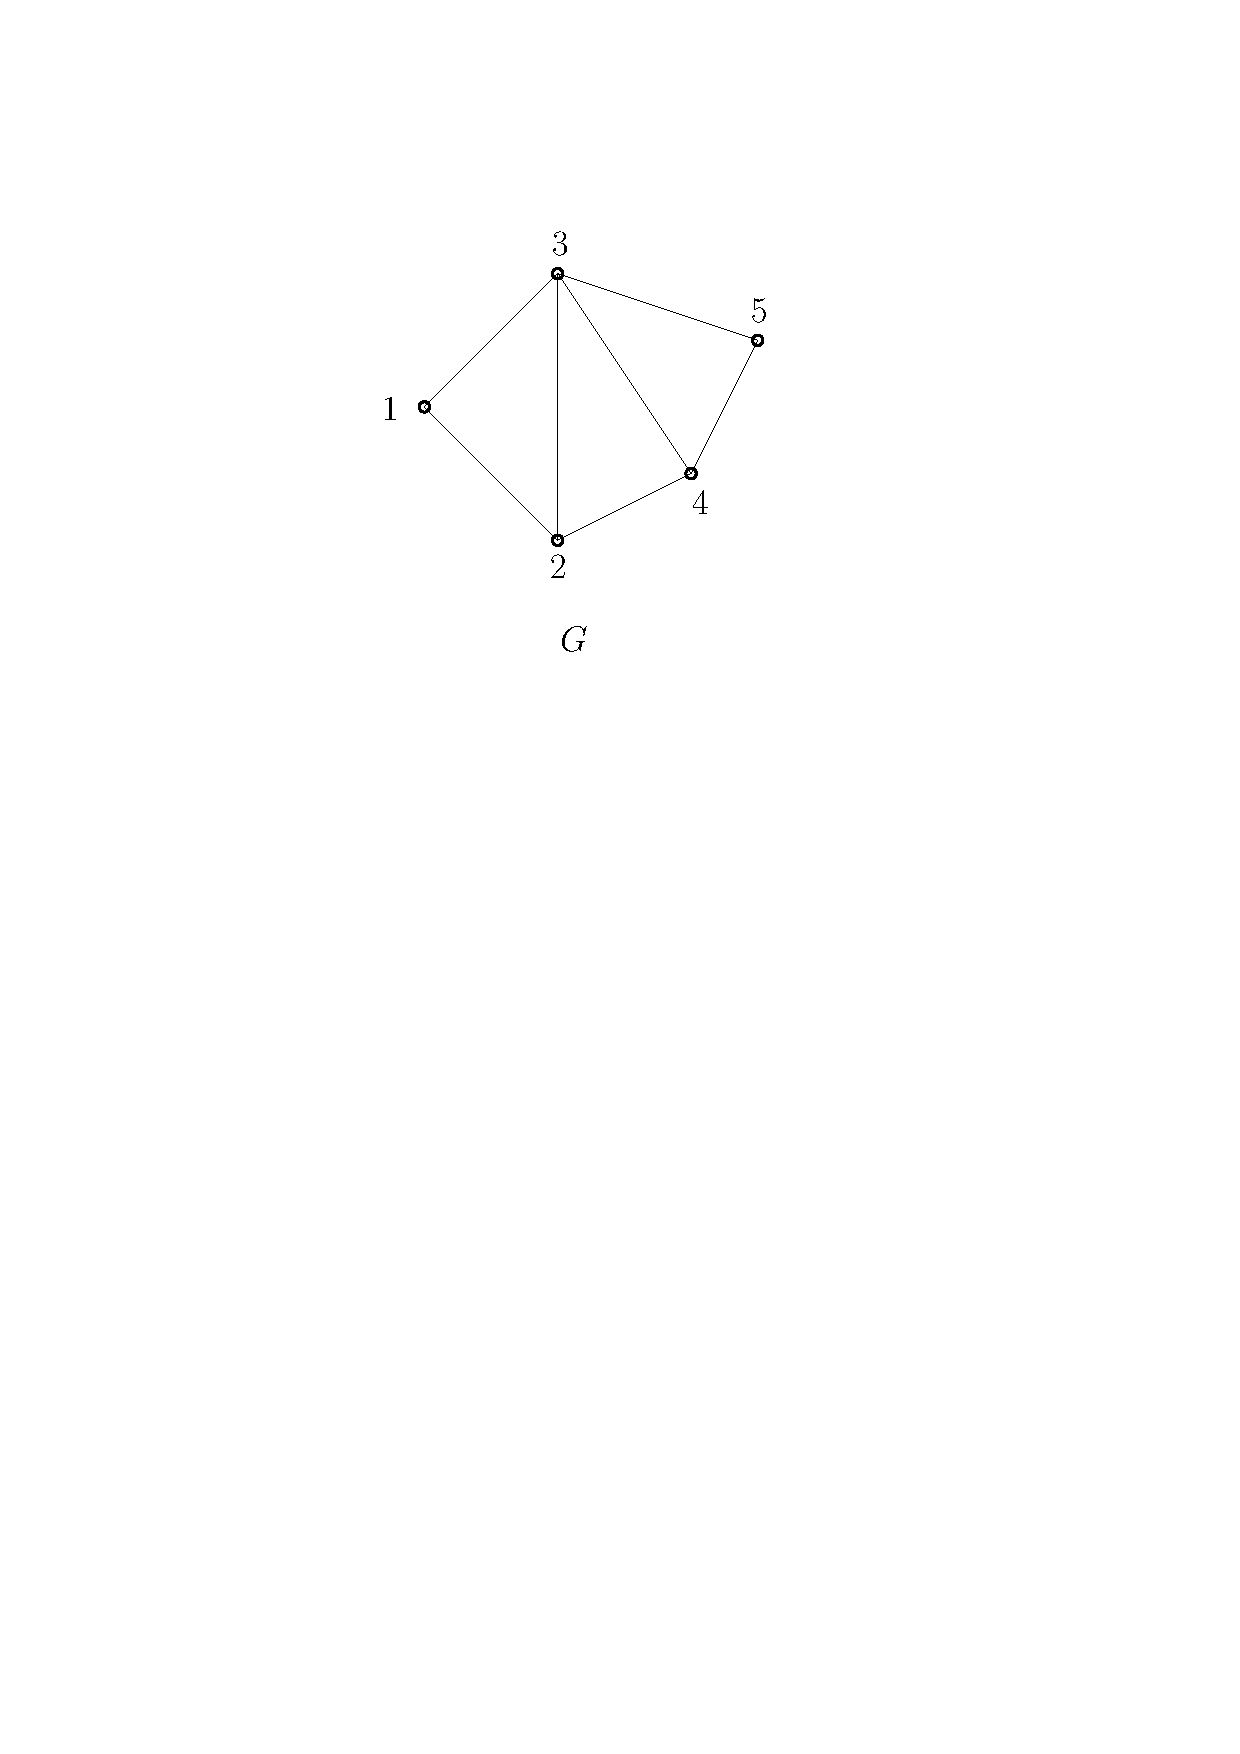
\includegraphics[height=32mm]{./artwork/tricnt-ex1}
    \end{center}
    
    \begin{center}
        3 triangles 
    \end{center}
}
%-------------------------------------------------------------
\myfrm{
    \xmybox{\blue{Dynamic} Triangle Counting}
    \vgap\vgap
    
    Design a structure to support  
    \myitems{
        \item \blue{update}$(\red{e})$: insert/delete $e$  
        \item \blue{query}: count the number of triangles 
    }
    
    \begin{center}
        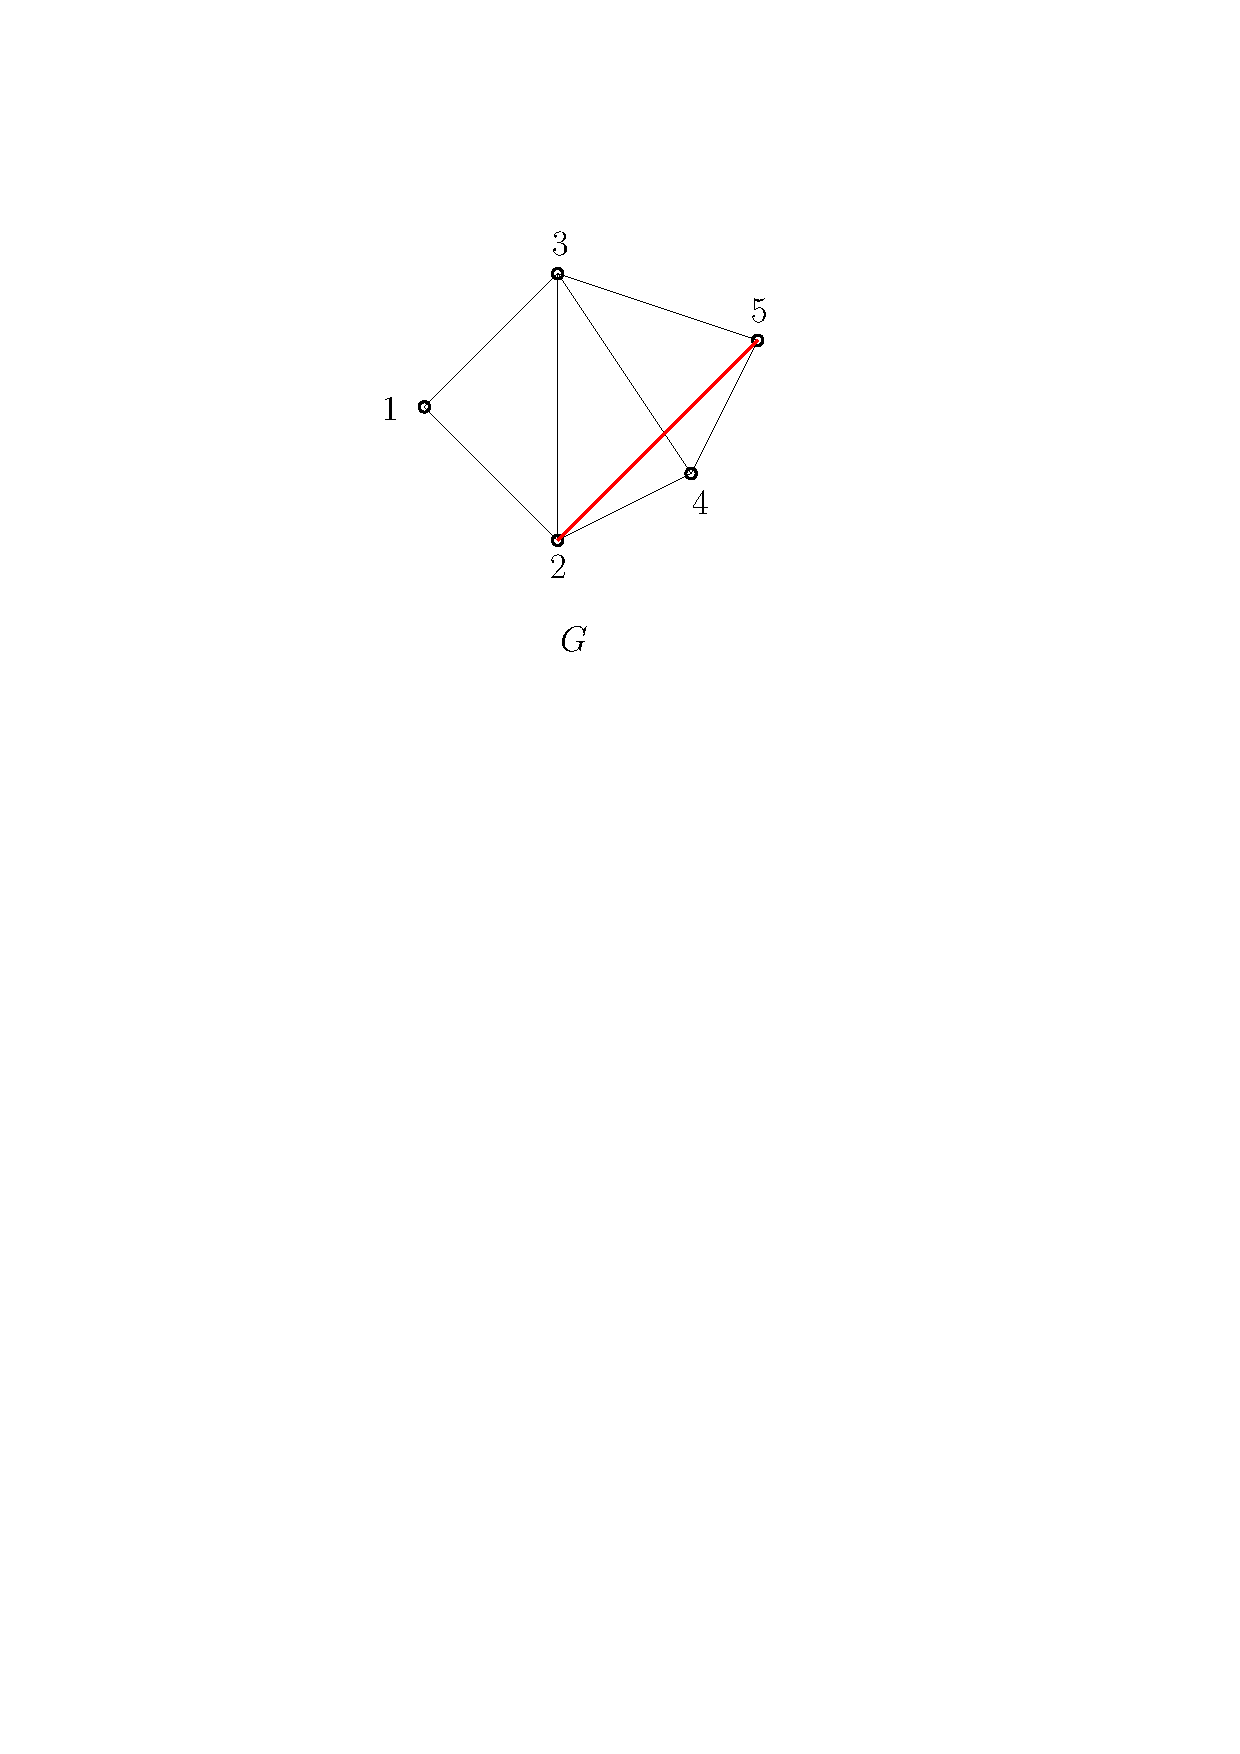
\includegraphics[height=32mm]{./artwork/tricnt-ex2}
    \end{center}
}
%-------------------------------------------------------------
\myfrm{
    \xmybox{OMv Conjecture}
    
    \begin{center}
        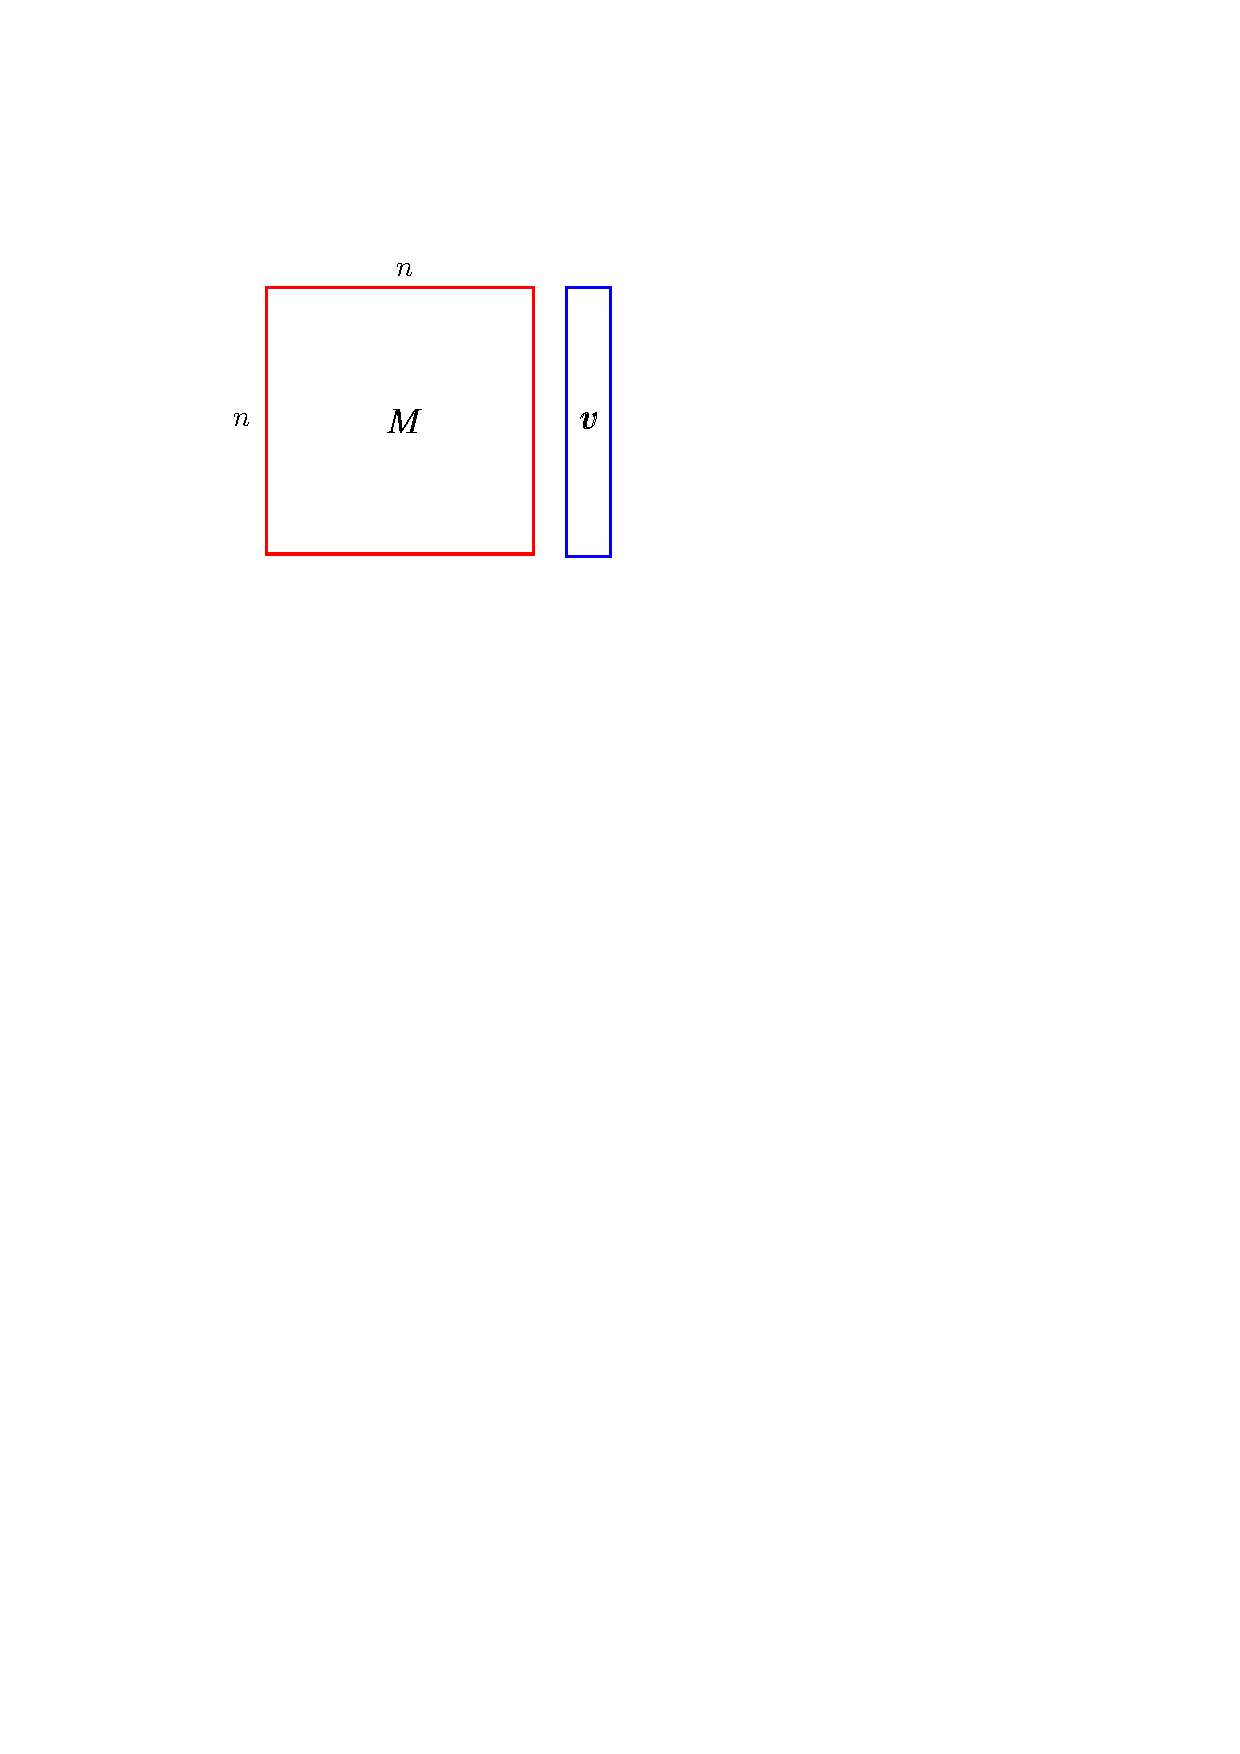
\includegraphics[height=32mm]{./artwork/omv}
    \end{center}
    
    
    \vgap 
    Need to calculate $\bm{M} \bm{v}_i$ for $i = 1, 2, ..., n$. \\ 
    Can do $O(n^{3-\delta})$? 
}
%-------------------------------------------------------------
\myfrm{
    \xmybox{Dynamic Triangle Counting}
    
    \vgap\vgap
    
    \cbox{red}{
        \blue{Thm 1} Subject to the OMv conjecture:
        \myitems{   
            \item either update needs $\Omega(\sqrt{m})$ time 
            \item or a query needs $\Omega(m)$ time. 
        }
    }
}
%-------------------------------------------------------------
\myfrm{
    \xmybox{\bred{Approximate} \blue{Dynamic} Triangle Counting}
    \vgap\vgap
    
    Design a structure to support  
    \myitems{
        \item \blue{update}$(\red{e})$: insert/delete $e$  
        \item \blue{query}: count the number of triangles up to \red{relative error $\eps$} 
    }
    
    \begin{center}
        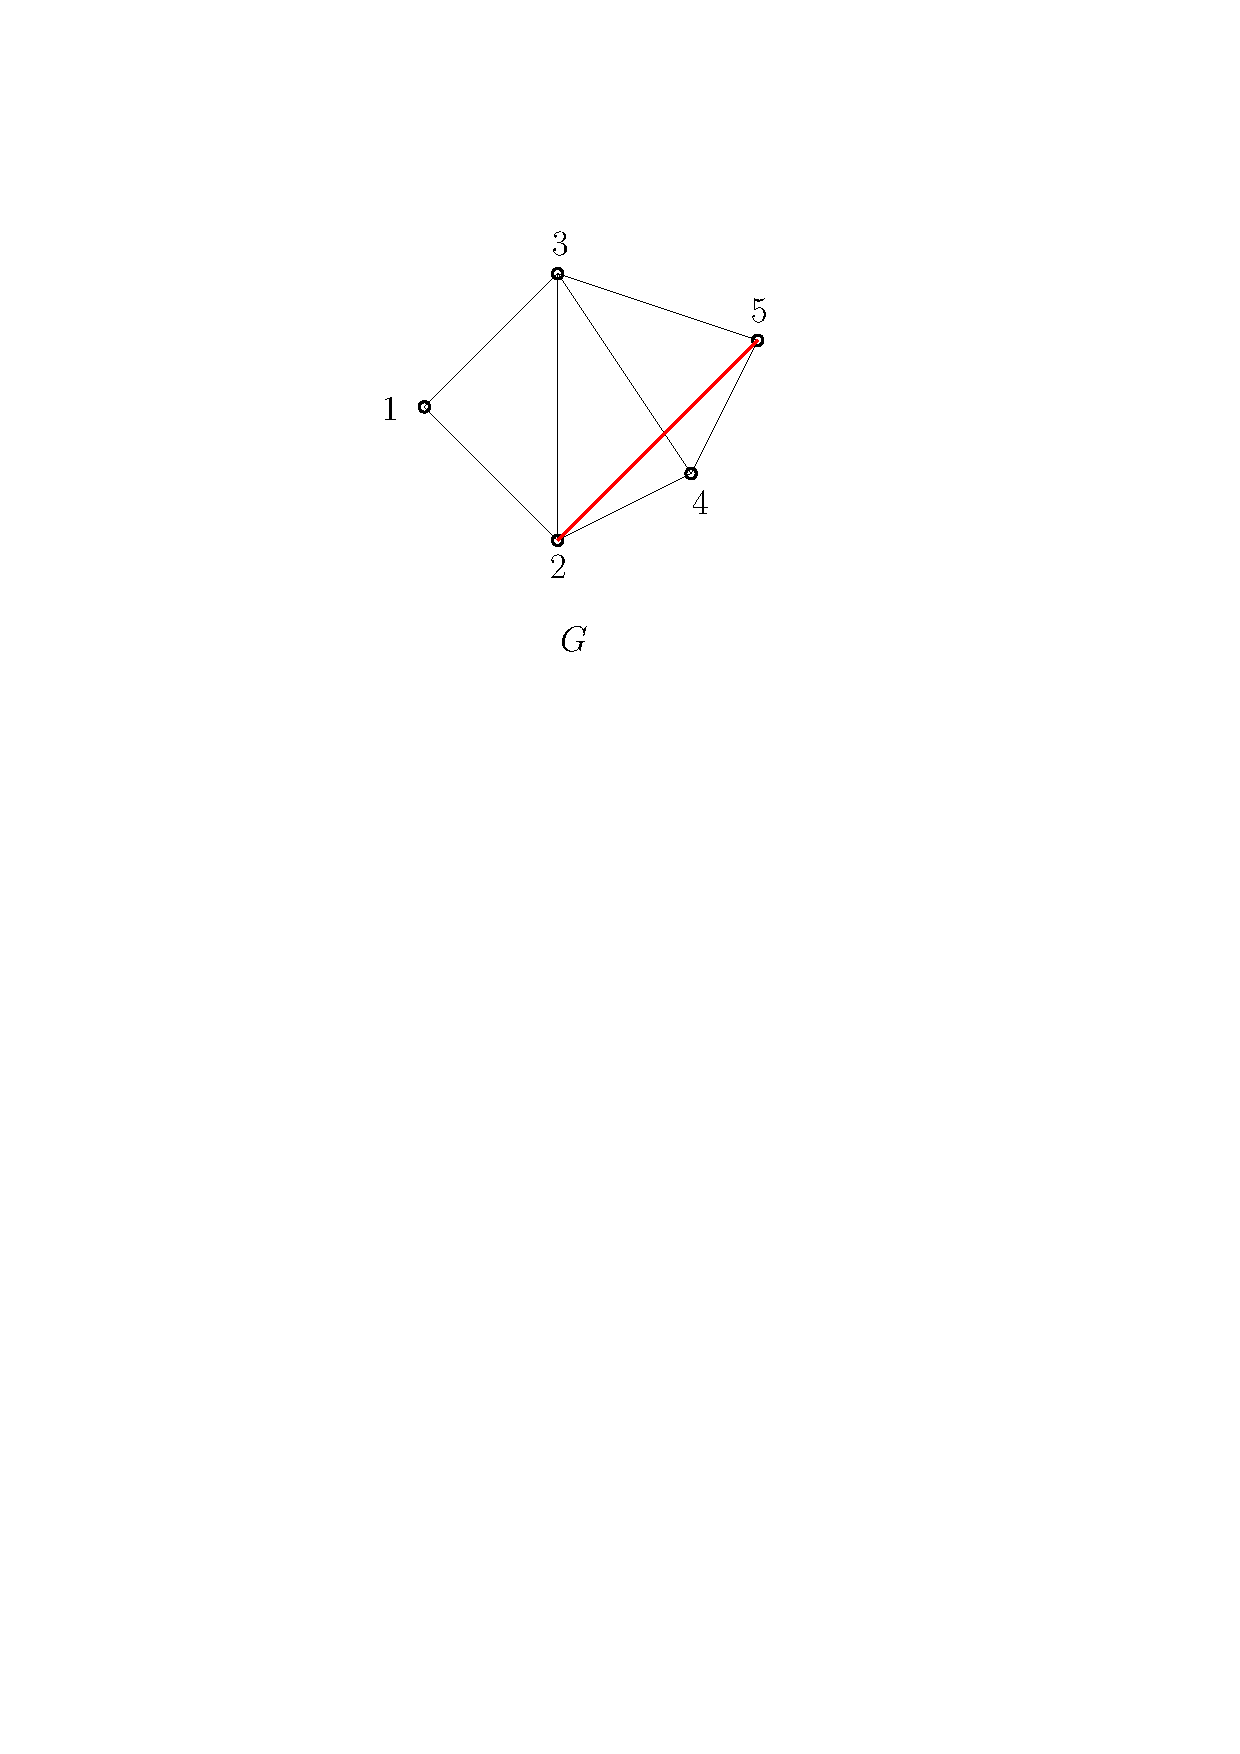
\includegraphics[height=32mm]{./artwork/tricnt-ex2}
    \end{center}
    
    \pause
    
    \cbox{red}{
        \blue{Thm 2} Subject to the OMv conjecture, for $\eps = 0.49$,
        \myitems{   
            \item either update needs $\Omega(\sqrt{m})$ time 
            \item or a query needs $\Omega(m)$ time. 
        }
    }
}
%-------------------------------------------------------------
\myfrm{
    \xmybox{\bred{Approximate} \blue{Dynamic} Triangle Counting}
    
    \vgap\vgap
    
    
    \cbox{blue}{
    \blue{$(\eps, \Gamma)$-guarantee}: 
    \myitems{
        \item $\red{\Gamma(m)}$: a function of $m$  
        \item If at least $\Gamma(m)$ triangles, \bred{relative} error $\eps$. \\ 
        Otherwise, \bred{absolute} error $\eps \cdot \Gamma(m)$. 
    }
    }
    
    \pause 
    
    \vgap
    
    \cbox{green}{
    Design a structure to support  
    \myitems{
        \item \blue{update}$(\red{e})$ 
        \item \blue{query}: give an estimate with the $(\eps, \Gamma)$-guarantee.
    }
    }
}
%-------------------------------------------------------------
\myfrm{
    \xmybox{\bred{Approximate} \blue{Dynamic} Triangle Counting}
    
    \vgap\vgap
    
    \cbox{red}{
        \blue{Thm 3} [Lu and Tao'21] \\
        Subject to the OMv conjecture, for $\eps = 0.49$,
        \myitems{   
            \item either update needs $\Omega(\fr{\sqrt{m}}{\red{\Gamma(m)}})$ time 
            \item or a query needs $\Omega(m^{2/3})$ time. 
        }
    }
    
    \pause 
    
    \cbox{green}{
        \blue{Thm 4} [Lu and Tao'21] \\
        Can do $\tO(\fr{\sqrt{m}}{\red{\Gamma(m)}})$ per update and $O(1)$ per query for any constant $\eps > 0$. 
    }
}
%-------------------------------------------------------------
\begin{frame}
\begin{small}
   
   \begin{center}
       \mybox[green]{THANK YOU}
   \end{center} 
   
\end{small}
\end{frame}
%-------------------------------------------------------------
\end{document} 
